%\documentclass[review,twocolumn,3p]{elsarticle}
\documentclass[preprint,twocolumn,3p]{elsarticle}
\usepackage{lineno,hyperref}
\modulolinenumbers[5]
\journal{Nuclear Instruments and Methods in Physics Research A}
\newcommand{\gx}{\textsc{GlueX}}

%%%%%%%%%%%%%%%%%%%%%%%
%% Elsevier bibliography styles
%%%%%%%%%%%%%%%%%%%%%%%
%% To change the style, put a % in front of the second line of the current style and
%% remove the % from the second line of the style you would like to use.
%%%%%%%%%%%%%%%%%%%%%%%

%% Numbered
%\bibliographystyle{model1-num-names}

%% Numbered without titles
%\bibliographystyle{model1a-num-names}

%% Harvard
%\bibliographystyle{model2-names.bst}\biboptions{authoryear}

%% Vancouver numbered
%\usepackage{numcompress}\bibliographystyle{model3-num-names}

%% Vancouver name/year
%\usepackage{numcompress}\bibliographystyle{model4-names}\biboptions{authoryear}

%% APA style
%\bibliographystyle{model5-names}\biboptions{authoryear}

%% AMA style
%\usepackage{numcompress}\bibliographystyle{model6-num-names}

%% `Elsevier LaTeX' style
\bibliographystyle{elsarticle-num}
%%%%%%%%%%%%%%%%%%%%%%%

\begin{document}

\begin{frontmatter}
\title{The \gx{} Start Counter Detector}	
\title{Design, Construction, \& Performance of The GlueX Start Counter Detector}
\author[jlab,fiu]{E. Pooser}
\author[jlab]{F. Barbosa}
\author[fiu]{W. Boeglin\corref{correspondingauthor}}
\cortext[correspondingauthor]{Corresponding Author}
\ead{boeglinw@fiu.edu}
\author[jlab]{C. Hutton}
\author[jlab]{M. Ito}
\author[fiu]{M. Kamel}
\author[fiu]{A. LLodra}
\author[jlab]{S. Taylor}
\author[fiu]{C. Yero}
\author[jlab]{B. Zihlmann}
\address[jlab]{Thomas Jefferson National Accelerator Facility, Newport News, VA 23606, USA}
\address[fiu]{Florida International University, Miami, FL, 33199, USA}
\begin{abstract}
The design, fabrication, calibration, and performance of the \gx{} Start Counter detector is described.  The Start Counter can operate at photon intensities up to $\mathrm{10^{8}\gamma/s}$ in the coherent peak and provides a range of timing resolutions of $\mathrm{450-700\ ps\ (FWHM)}$ thus providing successful identification of 500~MHz photon beam buckets to within than 94\% accuracy. Furthermore, the Start Counter provides excellent solid angle coverage, $\sim 90 \%\ \mathrm{of}\ 4 \pi\ \mathrm{hermeticity}$, a high degree of segmentation for background rejection, and can be utilized in the level 1 trigger for the experiment.  It consists of a cylindrical array of 30 thin scintillators with pointed ends that bend towards the beam at the downstream end. Magnetic field insensitive silicon photomultiplier detectors were selected as the readout system.
\end{abstract}
\begin{keyword}
GlueX \sep Flash ADC \sep F1 TDC \sep Plastic Scintillator \sep Silicon Photomultiplier \sep Multi-Pixel Photon Counter \sep Time of Flight \sep Trigger \sep Particle Identification
\end{keyword}
\end{frontmatter}

\linenumbers
\begingroup
\let\clearpage\relax
\section{Introduction}

% 
The \gx{} experiment, staged in Hall D at the Thomas Jefferson National Accelerator Facility (TJNAF), primarily aims to study the 
%rich 
spectrum of photo-produced mesons with unprecedented statistics.  The coherent bremsstrahlung technique is implemented to produce a linearly polarized photon beam incident on a liquid $\mathrm{H_{2}}$ target. A Start Counter detector was fabricated to properly identify the photon beam buckets and to provide accurate timing information. %WB edited
\section{Design} \label{sec:design}

In this section we discuss the details of the \gx{} Start Counter design.  The general engineering specifics pertaining to the scintillators, support structure, detector readout system and electronics are discussed.

\subsection{Overview} \label{sec:design_overview}
The Start Counter (ST) detector, seen in Fig.~\ref{fig:sttargetiso}, surrounds a 30~cm long super cooled liquid $\mathrm{H_{2}}$ target while providing $\sim 90 \%\ \mathrm{of\ 4 \pi}$ solid angle coverage relative to the target center.
	\begin{figure}[!htb]
		\centering
		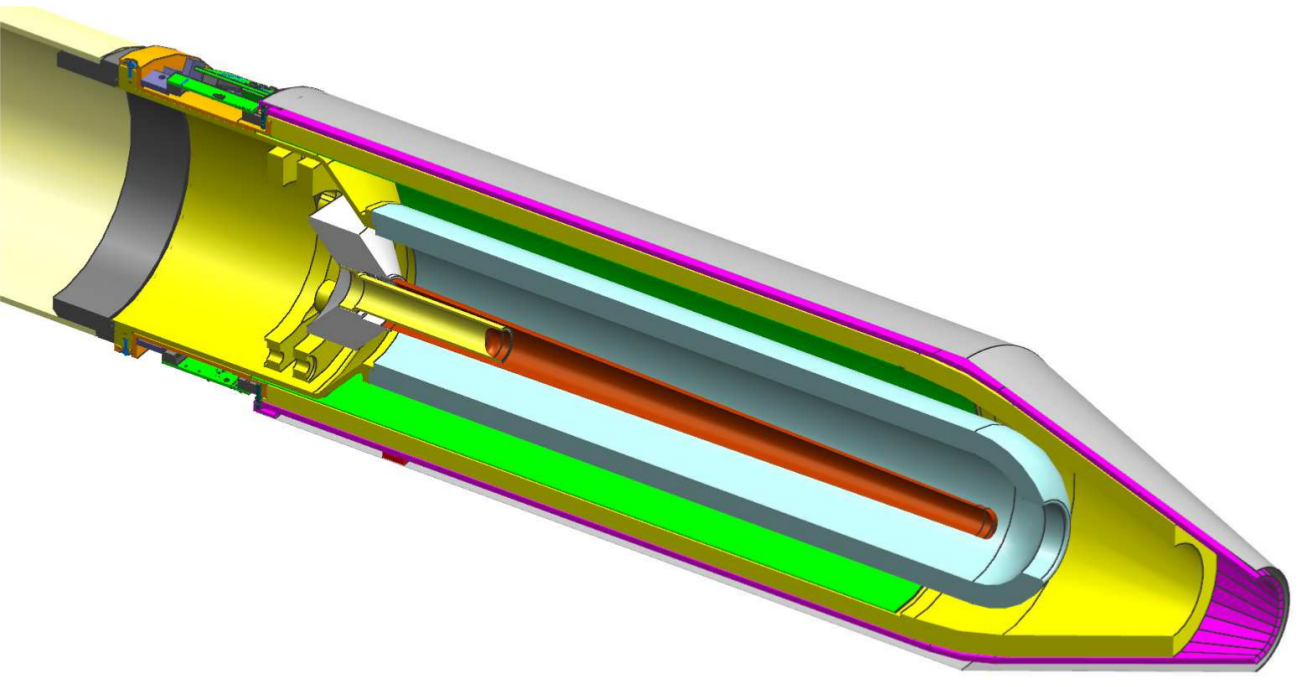
\includegraphics[width=1.0\columnwidth]{design/figs/st_target_iso}
		\caption{The \gx{} Start Counter mounted to the liquid $\mathrm{H_2}$ target.}
		\label{fig:sttargetiso}
	\end{figure}
The primary purpose of the ST detector is, in coincidence with the tagger, to properly identify the photon beam bucket associated with detected particles produced by linearly polarized photons incident on the target. It is designed to operate at tagged photon intensities of up to $10^{8}\,\mathrm{\gamma/s}$ in the coherent peak.  Moreover, the ST has a high degree of segmentation for background rejection, is utilized in particle identification, and is a primary component of the level 1 trigger of the \gx{} experiment during high luminosity running\cite{pooser16}.

The ST detector consists of an array of 30 scintillators with pointed ends that bend towards the beam at the downstream end. 
	\begin{figure}[!htb]
		\centering
		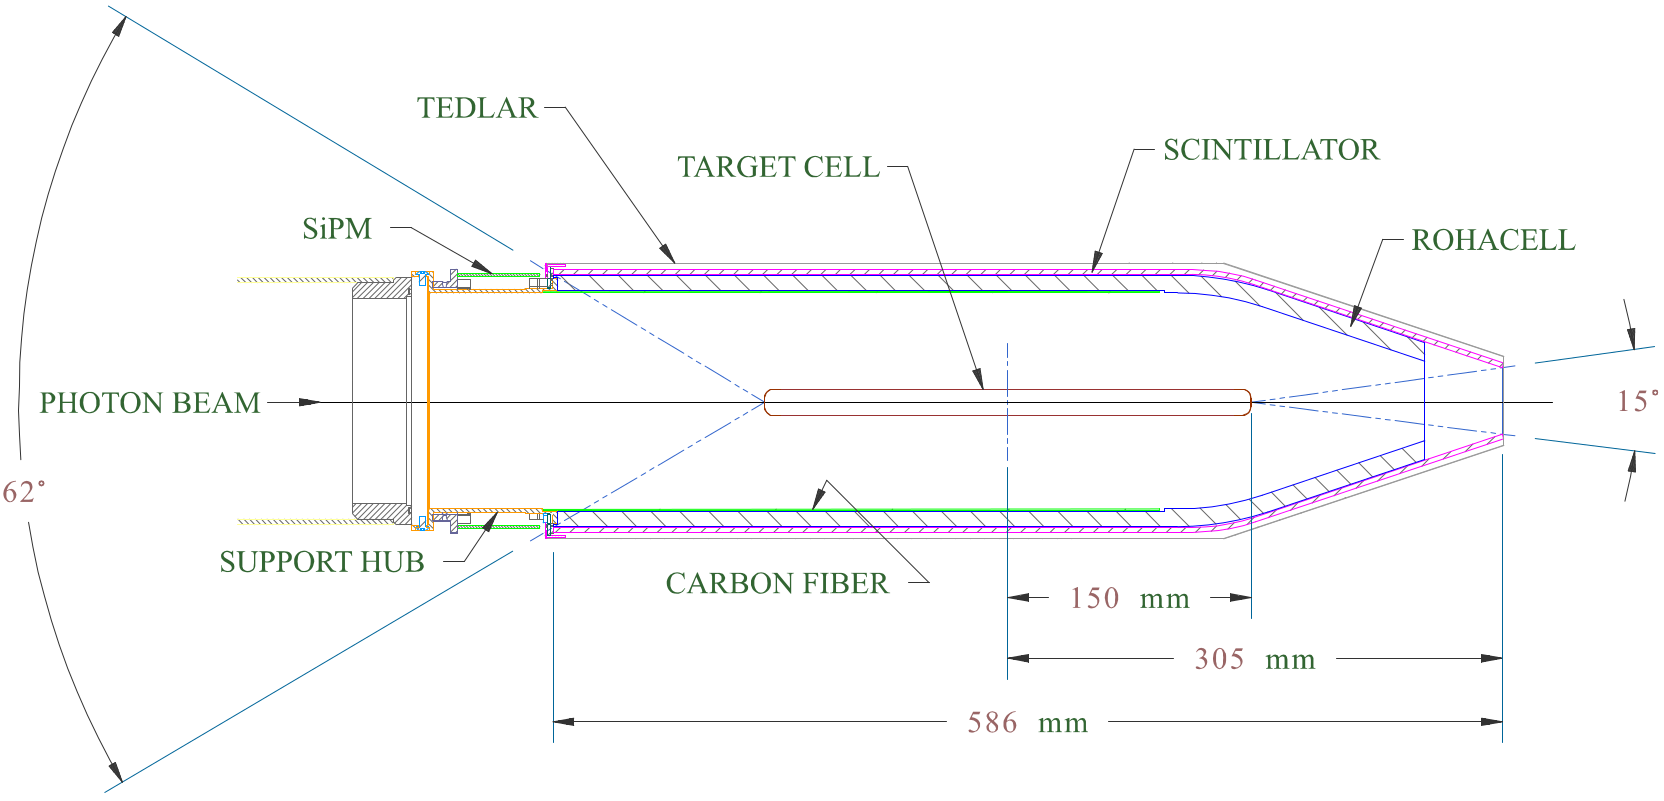
\includegraphics[width=1.0\columnwidth]{design/figs/st_2d_labels}
		\caption{Labeled 2-D cross section of the Start Counter detector.}
		\label{fig:st2dlabels}
	\end{figure}
EJ-200 scintillator material from Eljen Technology\cite{eljen}, which has a decay time of 2.1~ns and a long attenuation length\cite{ej200_specs}, was selected for this application.  The amount of support structure material was kept to an absolute minimum in the active region of the detector and is made up of low density Rohacell\cite{rohacell}. Silicon Photomultiplier (SiPM) detectors were selected as the readout system. The detectors are not affected by the high magnetic field produced by the superconducting solenoid magnet. Moreover, the SiPMs were placed as close as possible to the upstream end of each scintillator element, thereby minimizing the loss of scintillation light\cite{pooser16}.

\subsection{Scintillator Paddles} \label{sec:design_paddles}

Each individual paddle of the Start Counter was machined from a long, thin,  EJ-200 scintillator bar that was diamond milled to be 600~mm in length, 3~mm thick, and $\mathrm{20 \pm 2\ mm}$ wide, by Eljen Technology.  Each scintillator was bent around a highly polished aluminum drum by applying localized infrared heating to the bend region.  The bent scintillator bars were then sent to McNeal Enterprises Inc.\cite{mcneal}, a plastic fabrication company, where they were machined to the desired geometry illustrated in Fig.~\ref{fig:stpaddleiso}.
	\begin{figure}[!htb]
		\centering
		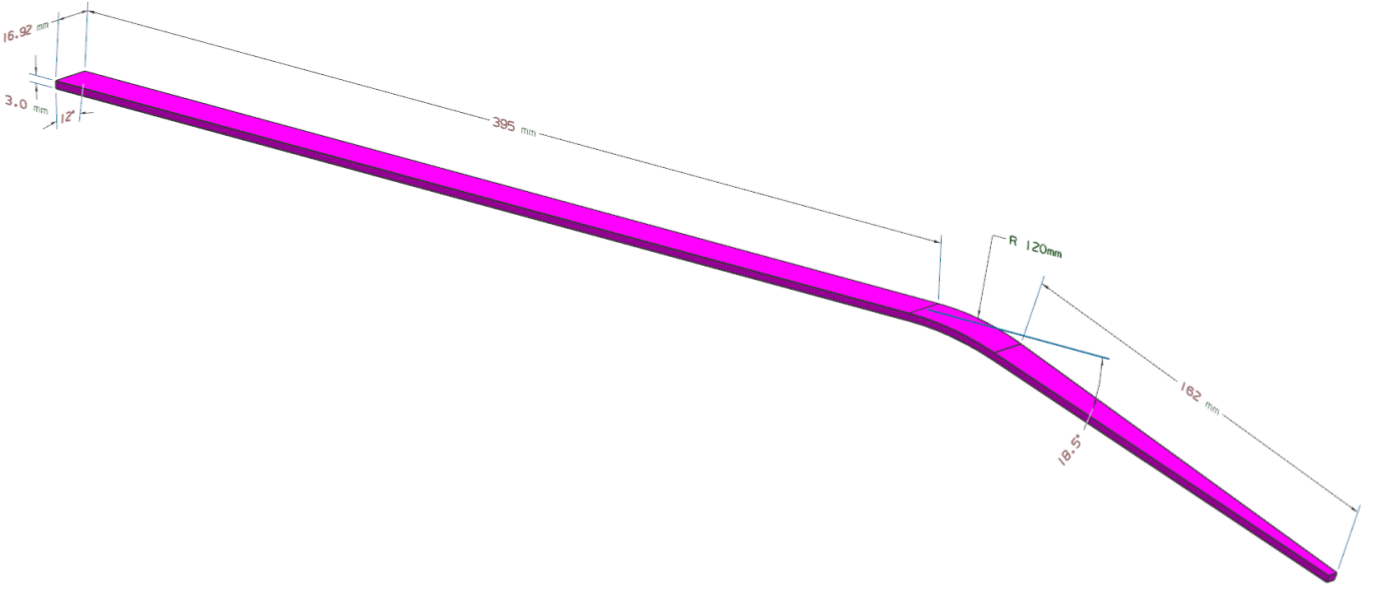
\includegraphics[width=1.0\columnwidth]{design/figs/st_paddle_iso}
		\caption{Start Counter single paddle geometry}
		\label{fig:stpaddleiso}
	\end{figure}

The paddles consist of three sections and are described from the upstream to the downstream end of the target.  The straight section is 39.5~cm in length while being oriented parallel to both the target cell and beamline.  The bend region is a $18.5^{\circ}$ arc of radius 120~cm and is downstream of the straight section. The tapered nose region is downstream of the target chamber and bends towards the beam line such that the tip of the nose is at a radial distance of 2~cm from the beam line.  

After the straight scintillator bar was bent to the desired geometry, the two flat surfaces that are oriented orthogonal to the wide, top and bottom, surfaces were cut at a $6^{\circ}$ angle.  During this process, the width of the top and bottom surfaces of the straight section were machined to be 16.92~mm and 16.29~mm wide respectively. Thus, each of the paddles may be rotated $12^{\circ}$ with respect to the paddle that preceded it so that they form a cylindrical shape with a conical end.  This geometrical design for the ST increases solid angle coverage while minimizing multiple scattering.  

\subsection{Support Structure} \label{sec:design_support}

The ST scintillator paddles are placed atop a low density Rohacell ($\mathrm{\rho = 0.075\ g/cm^{3}}$) foam support structure which envelopes the target vacuum chamber illustrated in Fig.~\ref{fig:sttargetiso}.
%	\begin{figure}[!htb]
%		\centering
%		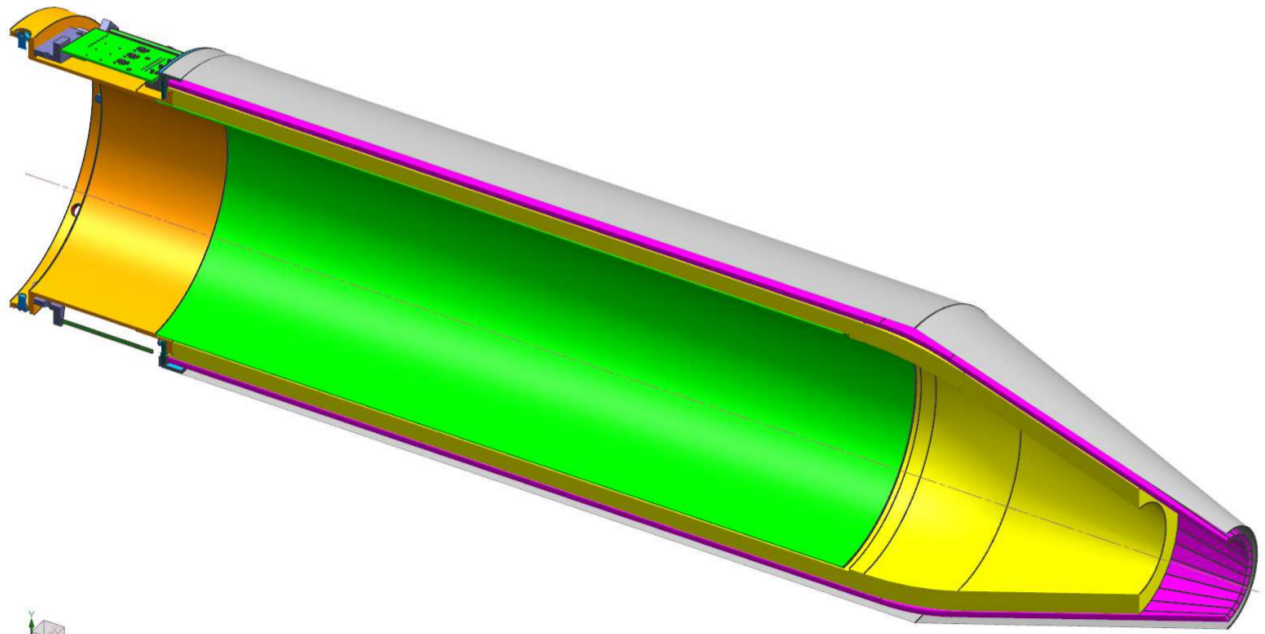
\includegraphics[width=1.0\columnwidth]{design/figs/st_iso}
%		\caption{Corss section of the Start Counter support structure.}
%		\label{fig:stiso}
%	\end{figure}
The Rohacell, which is 11~mm thick, is rigidly attached to the upstream support chassis and extends down the length of paddles however, not to include the last few centimeters of the conical nose section.  Glued to the inner diameter of the Rohacell support structure are 3 layers of carbon fiber ($\mathrm{\rho = 1.523\ g/cm^{3}}$) each of which are $\mathrm{650\ \mu m}$ thick.  A cross section of the ST can be seen in Fig.~\ref{fig:sttargetiso} where the carbon fiber is visible.  The carbon fiber provides additional support during the assembly process as well as long term rigidity.  

The various layers of material that comprise the ST support structure is illustrated in Fig.~\ref{fig:stmaterials}.
	\begin{figure}[!htb]
		\centering
		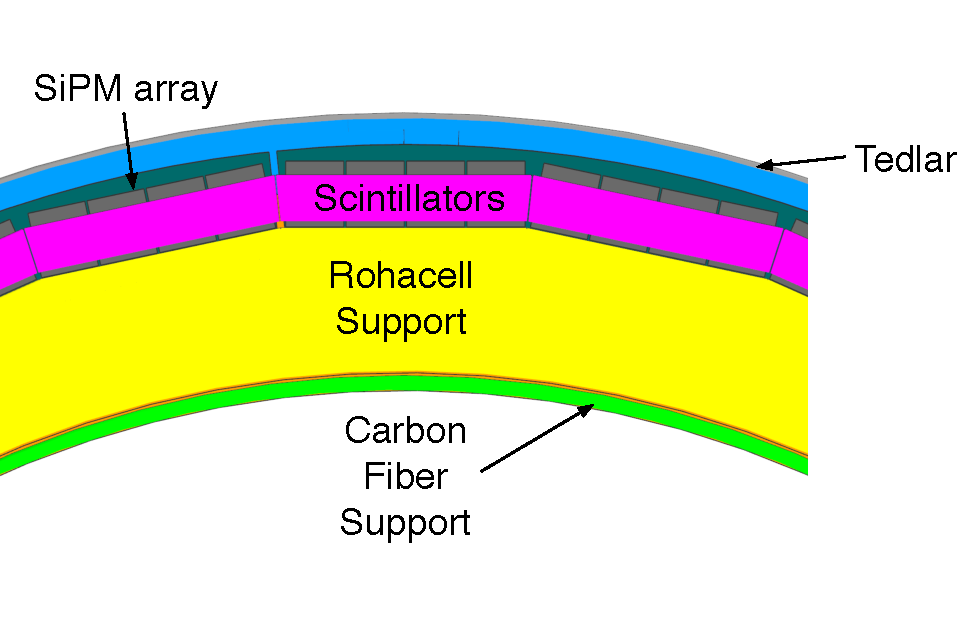
\includegraphics[width=1.0\columnwidth]{design/figs/st_materials}
		\caption{Start Counter materials.  Neon green corresponds to the 3 layers of carbon fiber, orange is the upstream support chassis, yellow is the Rohacell support structure, and magenta is the scintillator paddles.  The gray squares are the individual SiPM detectors, dark green is the readout printed circuit boards, blue is the light tightening collar, and the light-gray is Tedlar.}
		\label{fig:stmaterials}
	\end{figure}
In order to ensure that the detector was light-tight, a plastic collar was placed around the top of the SiPMs at the upstream end as seen in Fig.~\ref{fig:stmaterials}.  The collar served as a lip to which a cylindrical sheet of black Tedlar was taped too.  At the tip of the nose, a cone of Tedlar was then connected to the aforementioned cylindrical section.  To make the downstream end of the ST light-tight, another cone of Tedlar was taped to the nose of the inner Rohacell support structure and then attached to the top Tedlar cone layer. 


\subsection{SiPM Readout Detectors} \label{sec:design_sipms}

Each scintillator bar was read out using magnetic field insensitive Hamamatsu S10931-050P multi-pixel photon counters (MPPCs)\cite{hamamatsu}.  An individual $\mathrm{3 \times 3\ mm^2}$ MPPC, also known as a SiPM, in the aforementioned configuration is comprised of 3600 individual, $\mathrm{50 \times 50\ \mu m^2}$, Avalanche Photo-Diode (APD) pixel counters operating in Geiger mode. The signal output from each SiPM is the total sum of the outputs from all 3600 APD pixels\cite{sipm_spec}.  The scintillation light from an individual scintillator bar is collected by an array of four of these SiPMs.  Three groups of 4 SiPMs comprise what is referred to as the ``ST1'' of the readout system.

The SiPM detectors are housed in a ceramic case which is surface mounted to a custom fabricated printed circuit board (PCB).  The PCB is held in a fixed position while being attached to the lip of the upstream chassis.  The individual ST scintillators are coupled \emph{via} an air gap ($< 250 \mu m$) to groups of four SiPMs set in a circular arrangement as can be seen in Fig.~\ref{fig:st1_mounted}.  
% WB need to indicate the groups on this plot
% EP done.
	\begin{figure}[!htb]
		\centering
		%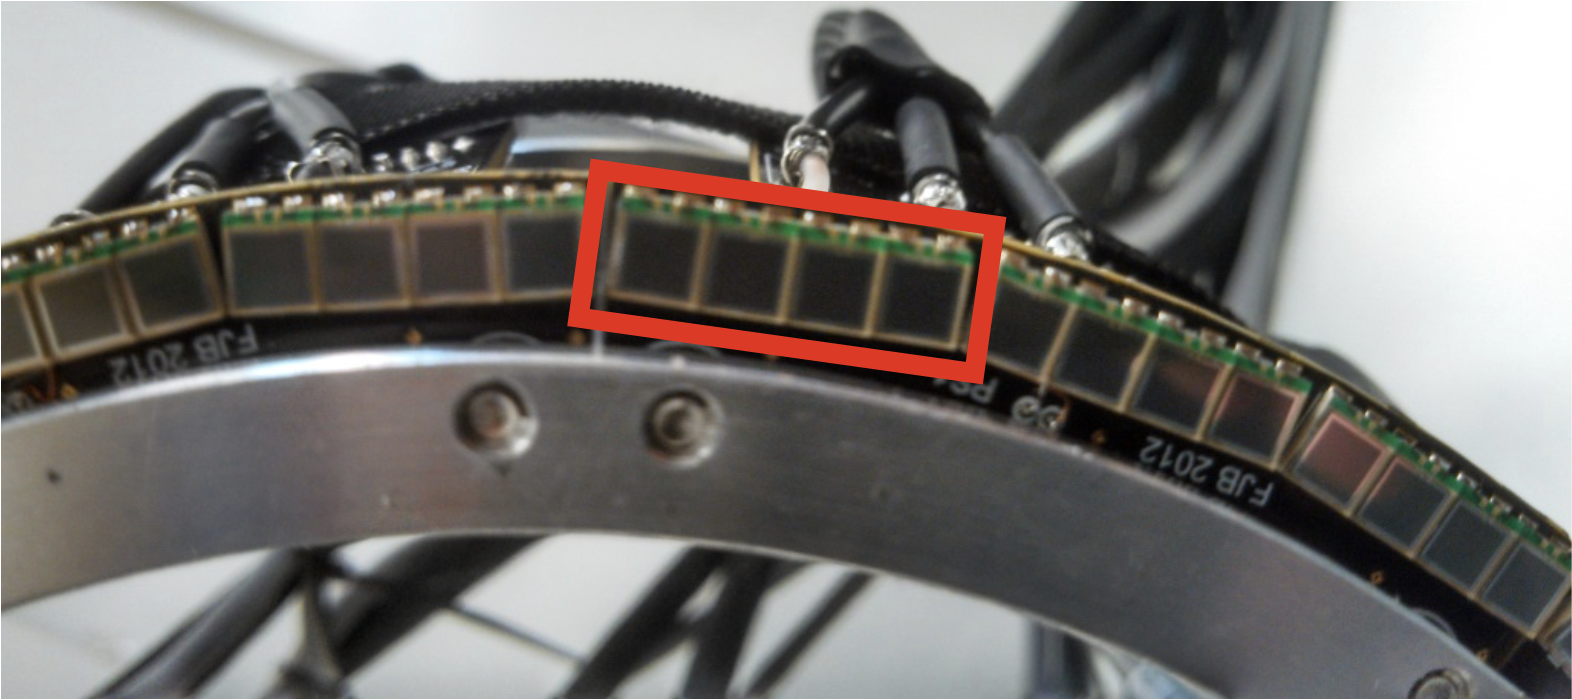
\includegraphics[width=1.0\columnwidth]{design/figs/st1_mounted_v2}
		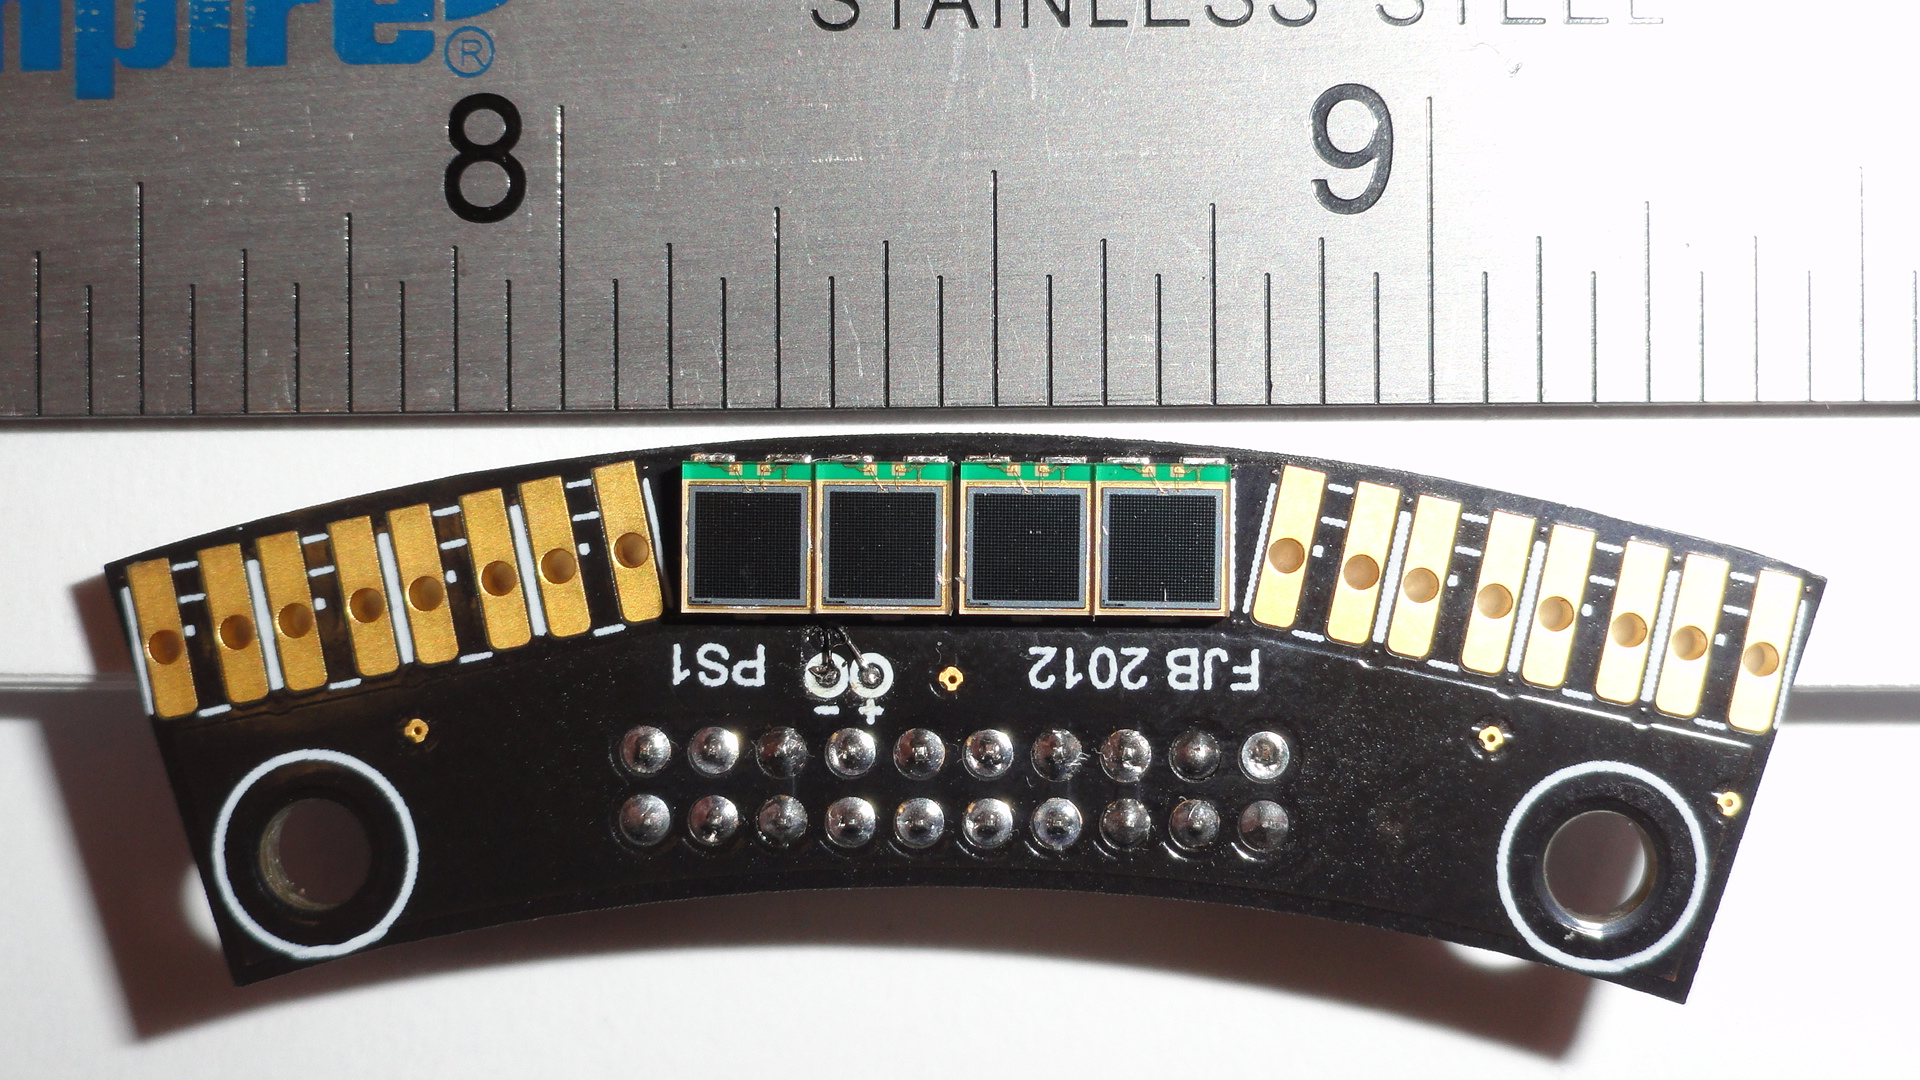
\includegraphics[width=1.0\columnwidth]{design/figs/st1_ruler}
		\caption{ST1 of Start Counter read out system. The ST1's are rigidly attached to the upstream support chassis.  Approximately 72\% of the scintillator light is collected at the upstream end.  Groups of 4 SiPM detectors are summed to readout a single scintillator paddle.  Three groups of 4 SiPM detectors are mounted to a single ST1 unit. The readout it comprised of 10 ST1 units.  The ruler shown is in inches.}
		\label{fig:st1_mounted}
	\end{figure}

\subsection{Readout Electronics} \label{sec:design_electronics}

The SiPMs reading out one individual paddle, are current summed prior to pre-amplification.  The output of each preamp is then split; buffered for the analog to digital converter (ADC) output, and amplified for the time to digital converter (TDC) output by a factor five relative to the ADC.  The ADC outputs are readout by JLab VME64x 250 MHz Flash ADC modules while the TDC outputs are input into JLab leading edge discriminators, followed by a high resolution 32 channel JLab VME64x F1TDC V2 module.  Furthermore, each group of four SiPMs utilizes a thermocouple for temperature monitoring. There are 120 SiPMs in total, for a total of 30 pre-amplifier channels as seen Fig.~\ref{fig:Start Counter Electronics}.

% WB this diagram needs more explanations of what the various parts do. Is every thing relevant ? Maybe indicate ST1 ST2 and ST3
% EP done.
	\begin{figure}[!htb]
		\centering
		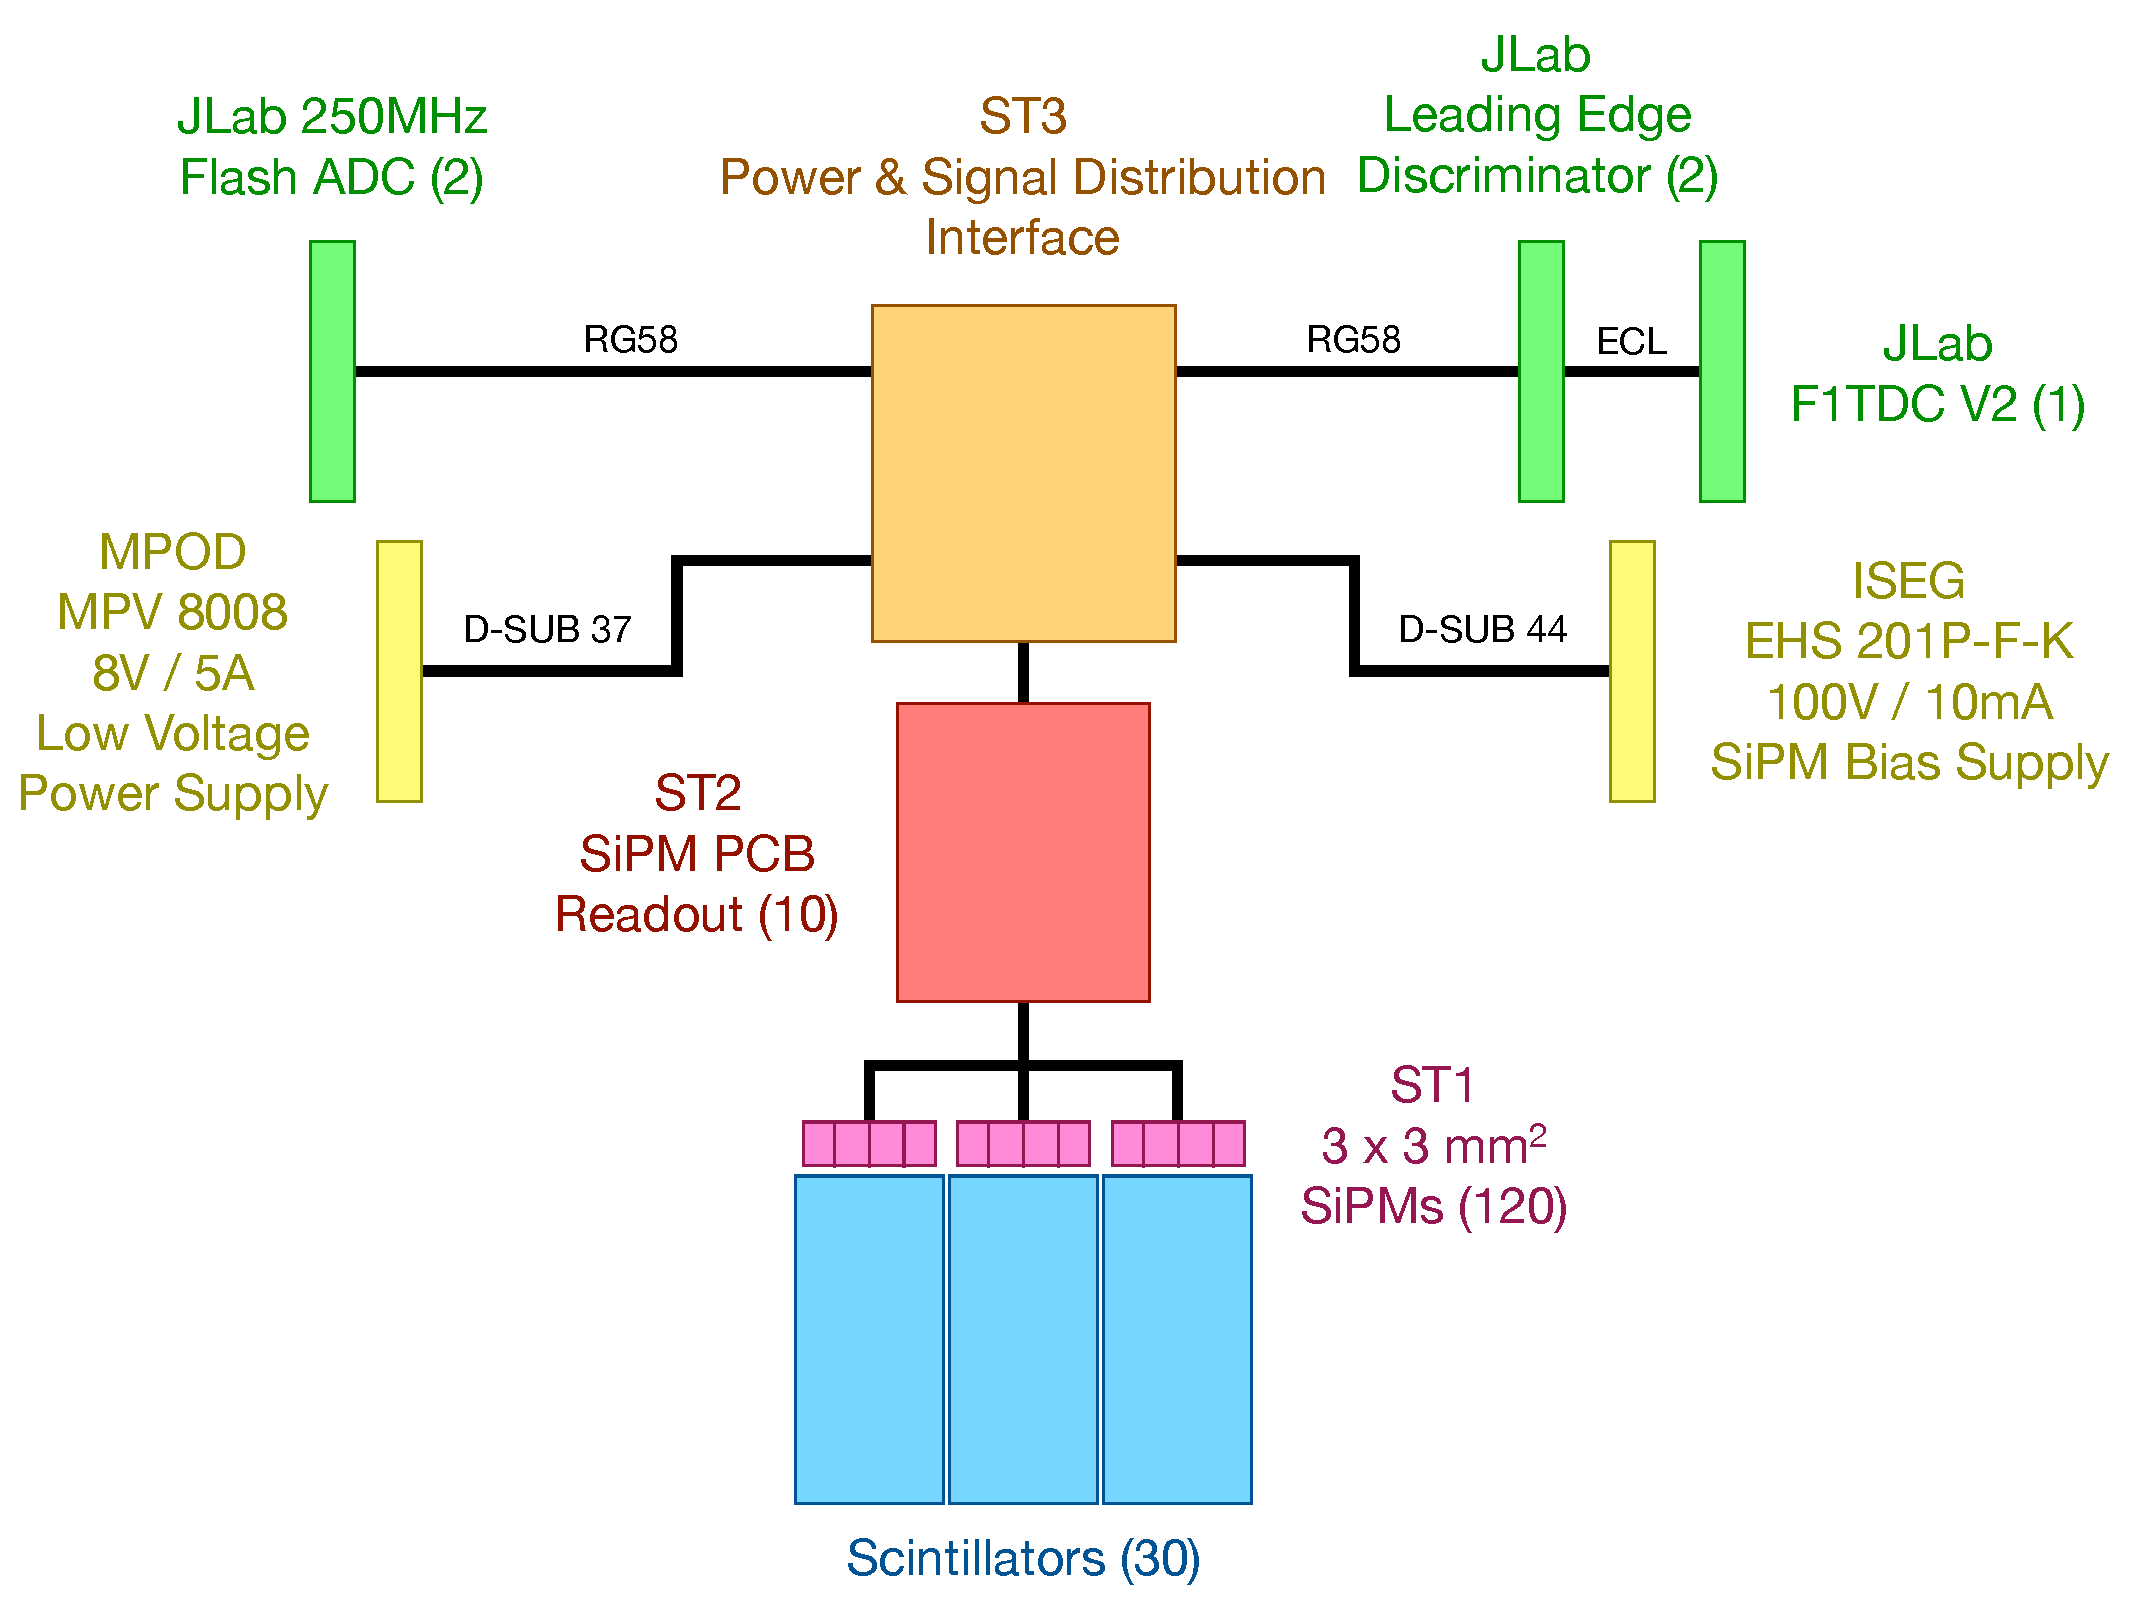
\includegraphics[width=1.0\columnwidth]{design/figs/st_electronics_diagram}
		\caption{Start counter readout electronics diagram.}
		\label{fig:Start Counter Electronics}
	\end{figure}

There are three components that comprise the ST detector readout system.  The first component (ST1), will collect light from three paddles individually and consists of 3 groups of 4 SiPMs as can be seen in Fig.~\ref{fig:st1_mounted}.  In order to fit the geometry of the 30 paddle design, one group of SiPM's is rotated by $12^{\circ}$ relative to the central group, while the other adjacent group is rotated by $-12^{\circ}$.  The ST1 implements the current sum and bias distribution for each group of 4 SiPMs.  It also has a thermocouple for temperature monitoring.  

The second component (ST2), seen in Fig.~\ref{fig:stfullreadout}, houses the signal processing electronics of the readout system.
	\begin{figure}[!htb]
		\centering
		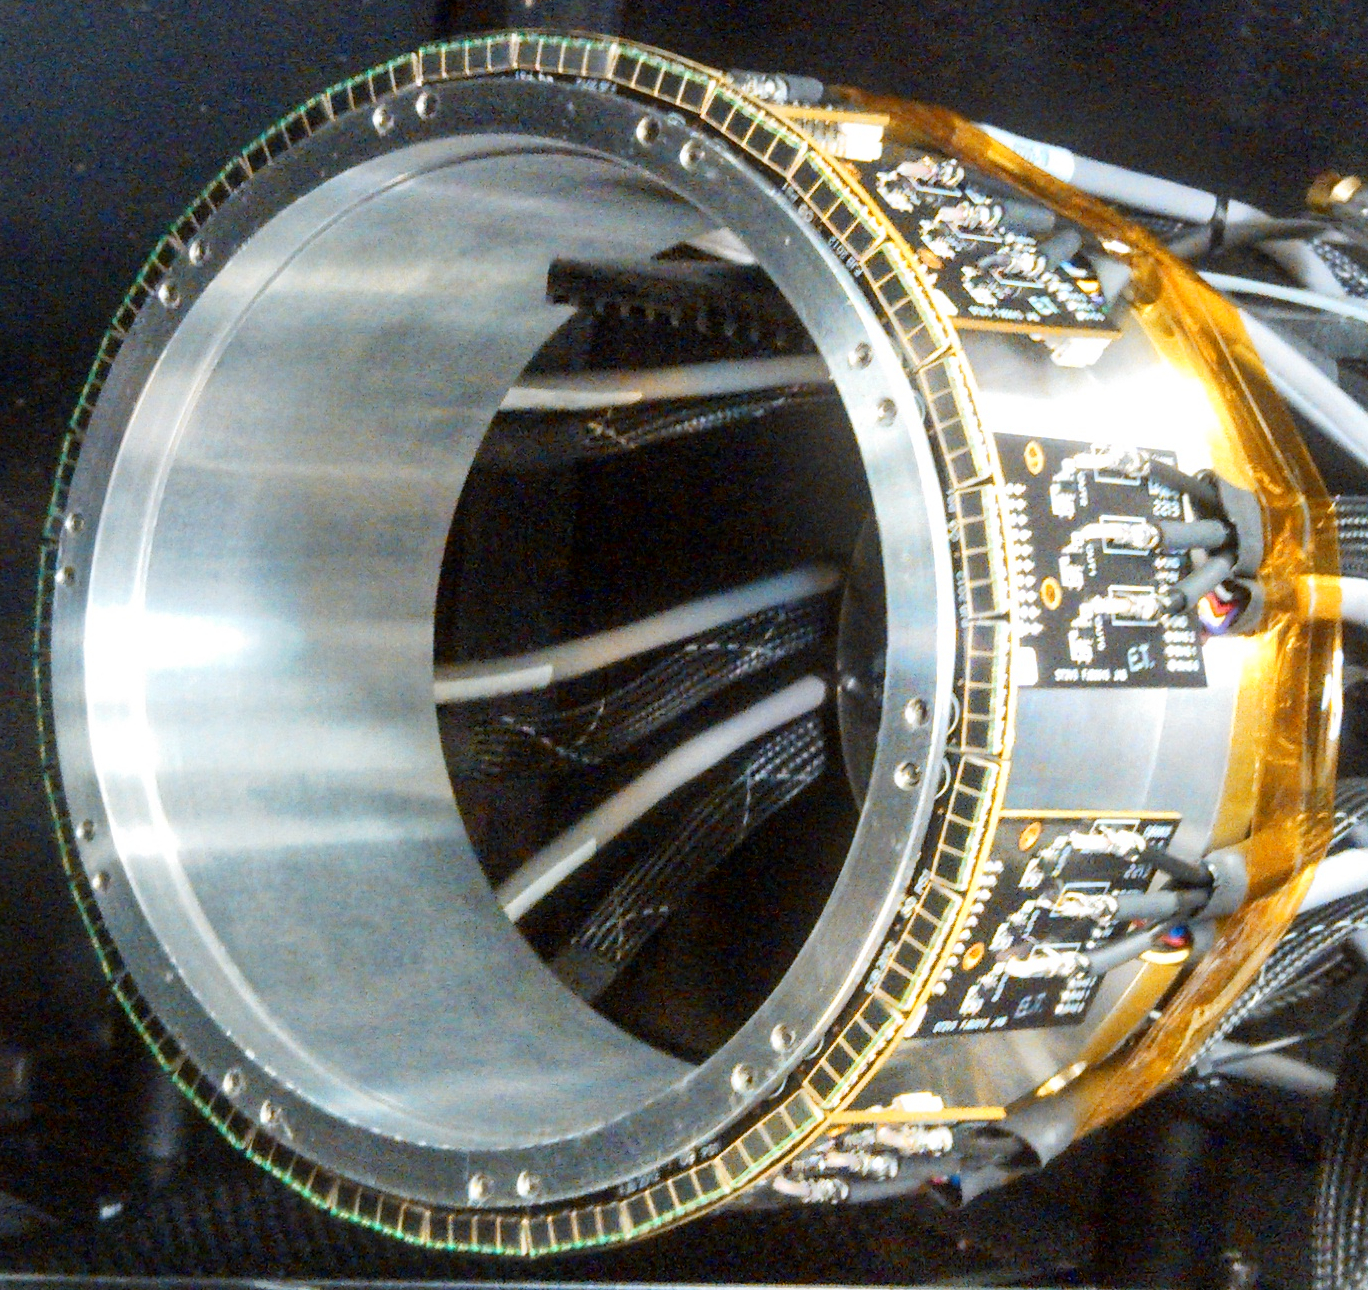
\includegraphics[width=1.0\columnwidth]{design/figs/st_full_readout_v3}
		\caption{Fully assembled ST readout system.  The ST2 unit is connected behind the ST1.  The full readout system is comprised of 10 ST2 units.}
		\label{fig:stfullreadout}
	\end{figure}
It has 3 channels of pre-amplifiers, 3 buffers, and 3 factor-five amplifiers.  Furthermore, it has 3 bias distribution channels with individual temperature compensation \emph{via} thermistors. % The ST2 is attached to the ST1 \emph{via} $90^{\circ}$ hermaphroditic connector.

% WB I am not sure a picture is needed here
% EP agreed.
%The third component of the readout system (ST3) seen in Fig.~\ref{fig:st3}, provides the interface to the power and bias supplies.
%	\begin{figure}[!htb]
%		\centering
%		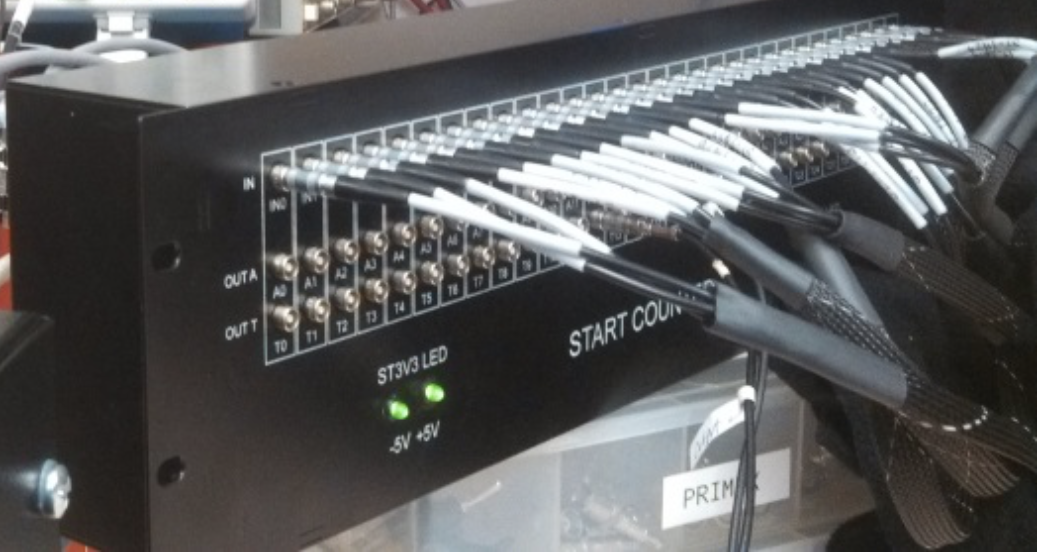
\includegraphics[width=1.0\columnwidth]{design/figs/st3}
%		\caption{Start counter ST3 readout system.}
%		\label{fig:st3}
%	\end{figure}
%It also routes the ADC and TDC outputs as well as the thermocouple output.  The ST3 connects to the ST2 \emph{via} a signal cable assembly seen in Fig.~\ref{fig:stfullreadout} and Fig.~\ref{fig:st3}.  The ST3 is installed upstream of the Start Counter and next to the beam pipe.
The third component of the readout system (ST3) provides the interface to the power and bias supplies.  It also routes the ADC and TDC outputs as well as the thermocouple output.  The ST3 is installed upstream of the Start Counter and next to the beam pipe. %WB edited
\section{GEANT4 Simulations} \label{sec:sim}

In this section, the Monte Carlo (MC) simulations that were conducted in order to better understand the performance and characteristics of scintillators machined to the nominal \gx{} Start Counter design are discussed.  The MC studies were performed with the use of the tool-kit GEANT4 which simulates the passage of particles through matter \cite{geant4_website}.  Comparisons are made with the data observed in experiments conducted on the bench in Sec.~\ref{sec:fab_test} and with beam data in Sec.~\ref{}.  

\subsection{Simulating a Simplified Model of the ST} \label{sec:sim_simple}

As discussed in Sec.~\ref{sec:design_paddles}, the ST scintillator paddles have a unique geometry in which the nose section tapers in width as the paddles approach the beam line at the downstream end.  This tapering effect results in a unique phenomenon in which the light output of the scintillator paddle begins to increase as the source moves further away from the readout detector.  At first, this phenomenon is completely contrary to what one might expect. In the traditional sense when the source moves further away from the end being readout, the photons have a larger effective path length and thus, have an increased probability in being lost for detection.  However, this is antithetical relative to what is observed on the bench and in experiment.

A primitive GEANT4 simulation was conducted to investigate the aforementioned phenomenon. For simplicity, only the two trapezoidal regions of a machined scintillator paddle were considered.  Namely, the wide straight section and the tapered nose section which are illustrated in the GEANT4 event display  seen in Fig. \ref{fig:beam_off}.
	\begin{figure}[!htb]
	\centering
	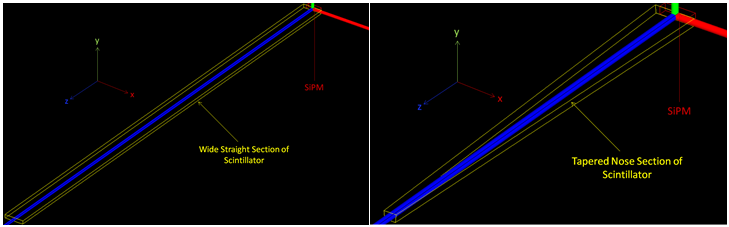
\includegraphics[width=1.0\columnwidth]{simulation/figs/beam_off}
	\caption{Simulated straight \& nose section geometries.  Shown is the GEANT4 event display.  Left: wide straight section.  Right: tapered nose section.  The sections have been oriented such that they are in the same coordinate system as defined in HallD.  The yellow lines are the scintillator boundaries, while the red lines are the boundaries of the SiPM.}
	\label{fig:beam_off}
	\end{figure}  

The EJ-200 scintillator material ($\rho=1.023~\mathrm{g/cc^{3}}$, $n = 1.58$) \cite{ej200_specs} was simulated with only one free parameter utilized to characterize the scintillator bar \textit{i.e.}, the reflectivity of the \textit{G4LogicalSkinSurface}, was set to 98\% so there remained some finite probability that photons could be lost in the scintillator medium.  Furthermore, the SiPM readout detector was placed at the upstream end of the two sections, seen in Fig. \ref{fig:beam_off}.  Moreover, the SiPM was constructed as a \textit{G4SensitiveDetector} made of Silicon with a 100\% detection efficiency.  The SiPM was constructed to have an active area of $\mathrm{3 \times 12~mm^2}$ which is identical to the readout system described in Sec.~\ref{sec:design_sipms}.

In order to simulate a charged particle traversing through the scintillator medium resulting in the production of photons along its path through the material, optical photons were generated inside the volume of the simulated scintillator material.  The scintillation yield was defined to be $\mathrm{10,000~ \gamma 's / 1~MeV}$ \cite{ej200_specs}. For visual purposes, Fig. \ref{fig:100_events} shows 100 optical photons being produced at the tip of the downstream end of the two sections of the simulated scintillator paddle.
	\begin{figure}[!htb]
	\centering
	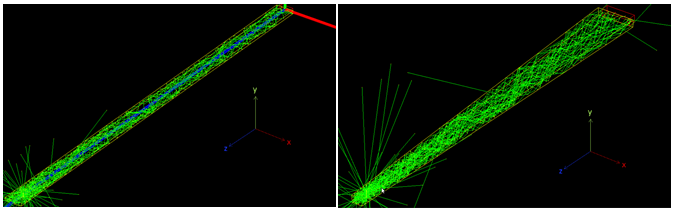
\includegraphics[width=1.0\columnwidth]{simulation/figs/100_events}
	\caption{100 Optical photons generated in the staight \& nose sections.  Left: wide straight section.  Right: tapered nose section.  The neon green lines are the paths of the optical photons.  It is clear that some photons do in fact escape the scintillator medium, while others are collected in the simulated SiPM detector.}
	\label{fig:100_events}
	\end{figure}

In order to sample the entirety of the two sections, 10,000 optical photons were generated at 16 different locations inside the medium of the scintillator. 
	\begin{figure}[!htb]
	\centering
	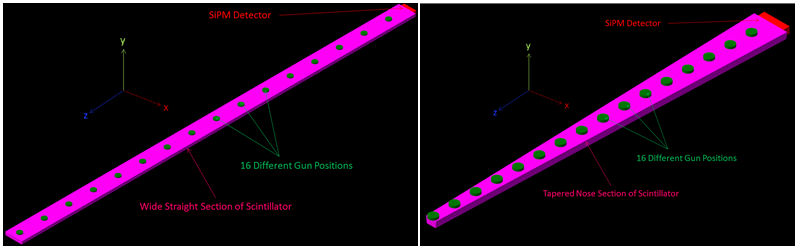
\includegraphics[width=1.0\columnwidth]{simulation/figs/gun_locations}
	\caption{Optical photon gun locations along the straight \& nose sections. Left: wide straight section.  Right: tapered nose section.  The magenta geometries indicate the scintillator boundaries of the two sections.  The red box is the sensitive SiPM detector, and the green cylinders represent the location of the 16 optical photon gun locations. The locations of the source were chosen to be equal distances apart relative to each of the two sections.}
	\label{fig:gun_locations}
	\end{figure}
The photon energies ranged between $0.5 - 3.0$ eV \cite{krane_ch7} and were generated randomly in $4\pi$ along a 3 mm path $(y-axis)$ in the scintillator medium.  The path was oriented orthogonal to the wide surface of the scintillator.  In essence, this simulates a charged particle traversing through the medium with a $\theta_{track} = 90^{\circ}$ in hall coordinates.  The number of photons collected by the SiPM at each of the 16 source locations is counted and correlated to the source location.  The results can be seen in Fig. \ref{fig:sim_results}.
	\begin{figure}[!htb]
	\centering
	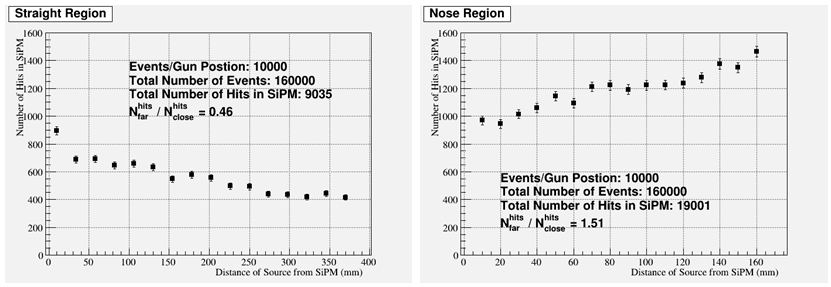
\includegraphics[width=1.0\columnwidth]{simulation/figs/sim_results}
	\caption{Simulation results for simplified two section scenario. The total number of photons which were collected by the SiPM detector at each of the 16 source locations is plotted against the sources distance from the sensitive detector. Left: wide straight section.  Right: tapered nose section.}
	\label{fig:sim_results}
	\end{figure}
From the data it is clear that the geometry of the nose section results in an improvement of light collection as the source moves further away from the readout detector.  In fact, there is a factor $\approx 1/2$ light loss observed in the straight section upon comparing the number of hits collected at the closest and furthest locations relative to the readout detector.  However, there is factor $\approx 3/2$ light gain observed in the nose region.  These results are primarily due to the tapering trapezoidal geometry in the nose section.  This phenomenon is not observed in the quasi-rectangular straight section as it exhibits a more conventional behavior. However, this behavior in the nose region is advantageous since the majority of forward going charged particles will traverse through the this region.

\subsection{Simulating Machined Scintillator Geometry} \label{sec:sim_mach}

Further simulations were conducted to simulate more realistically the effects of light collection that results from the ST scintillator geometry and optical surface quality.  The ST scintillator geometry was imported into GEANT4 from a Vectorworks CAD drawing utilizing the CADMesh utility \cite{cadmesh_g4} and is shown \textit{via} the GEANT4 event display in Fig. \ref{fig:pk_cadmesh}.
	\begin{figure}[!htb]
	\centering
	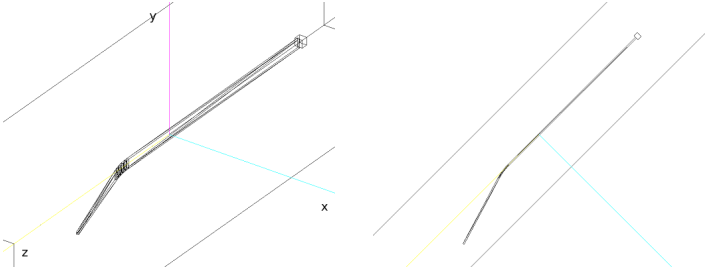
\includegraphics[width=1.0\columnwidth]{simulation/figs/pk_cadmesh}
	\caption{Scintillator geometry imported into GEANT4 utilizing CADMesh Utility.  The scintillator is  coupled to a SiPM detector.  Left: isometric view.  Right: top view.  The tapering of the nose section is clearly visible.}
	\label{fig:pk_cadmesh}
	\end{figure}
The SiPM was constructed as a $12 \times 12 \times\ 10\ \mathrm{mm^{3}}$ volume with a 100 $\mathrm{\mu m}$ air gap between it and the wide end of the straight section.  Furthermore, the volume surrounding the scintillator volume was air.  The EJ-200 scintillator material, SiPM silicon detector, and optical photons were defined in an identical manner discussed in Sec.~\ref{sec:sim_simple}.

To simulate the imperfections of the scintillator surfaces due to manufacturing and machining, an optical surface ``skin'' was defined.  The ``skin'' material was defined to be of they type ``dielectric-dielectric'' and made use of the UNIFIED physics model \cite{scint_surface_sim} to define an imperfect scintillator surface.  Both the transmission efficiency and reflection parameters were implemented as free parameters to study their various effects on light transmission..  

The UNIFIED model allows one to define the finish of the scintillator surface as \textit{polished}, \textit{ground}, or \textit{unified} and is illustrated in Fig.~\ref{fig:polished_vs_ground} \cite{scint_surface_sim}.
	\begin{figure}[tbph]
	\centering
	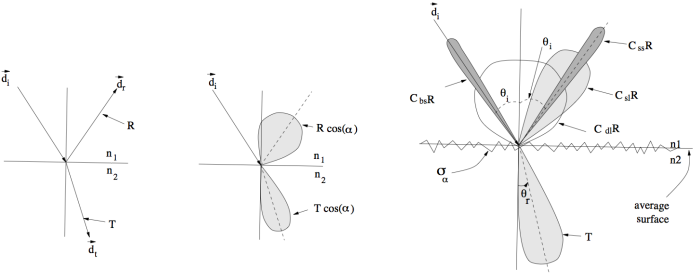
\includegraphics[width=1.0\columnwidth]{simulation/figs/polished_vs_ground}
	\caption{UNIFIED Model of scintillator surfaces.  Left: Polar plot of the radiant intensity of the polished (left) and ground (right) models.  Right: Polar plot of the radiant intensity in the UNIFIED model.}
	\label{fig:polished_vs_ground}
	\end{figure}

In the polished model, Fresnel reflection and refraction is assumed, where as the ground model allows for Lambertian reflection, Fresnel refraction, backscattering, as well as spike and lobe reflections.  The spike ($C_{ss}$) reflection parameter assumes the optical photons are reflected as if the surface was a perfect mirror.  The backscattering ($C_{bs}$) reflection parameter assumes the photon is reflected in the same direction of incidence.  The Lambertian ($C_{dl}$) reflection parameter assumes that the photons are reflected corresponding to a Lambertian distribution.  The lobe ($C_{sl}$) reflection parameter assumes that the photons will reflect based on the orientation of the micro-facet on the scintillator surface, where $\sigma_{\alpha}$ defined the standard deviation of the distribution of the micro-facets orientation \cite{scint_surface_sim}.  One caveat of the aforementioned models is that they assume identical parameters for the entire optical surface \cite{puneet_sim_wiki}.

As was done in section \ref{sec:sim_simple}, 10,000 optical photons were generated in the scintillator medium every 2.5 cm and the number of hits collected in the SiPM were recorded.  The results of these simulations are show in Fig. \ref{fig:transm_eff_vs_sig_alpha}.
	\begin{figure}[!htb]
	\centering
	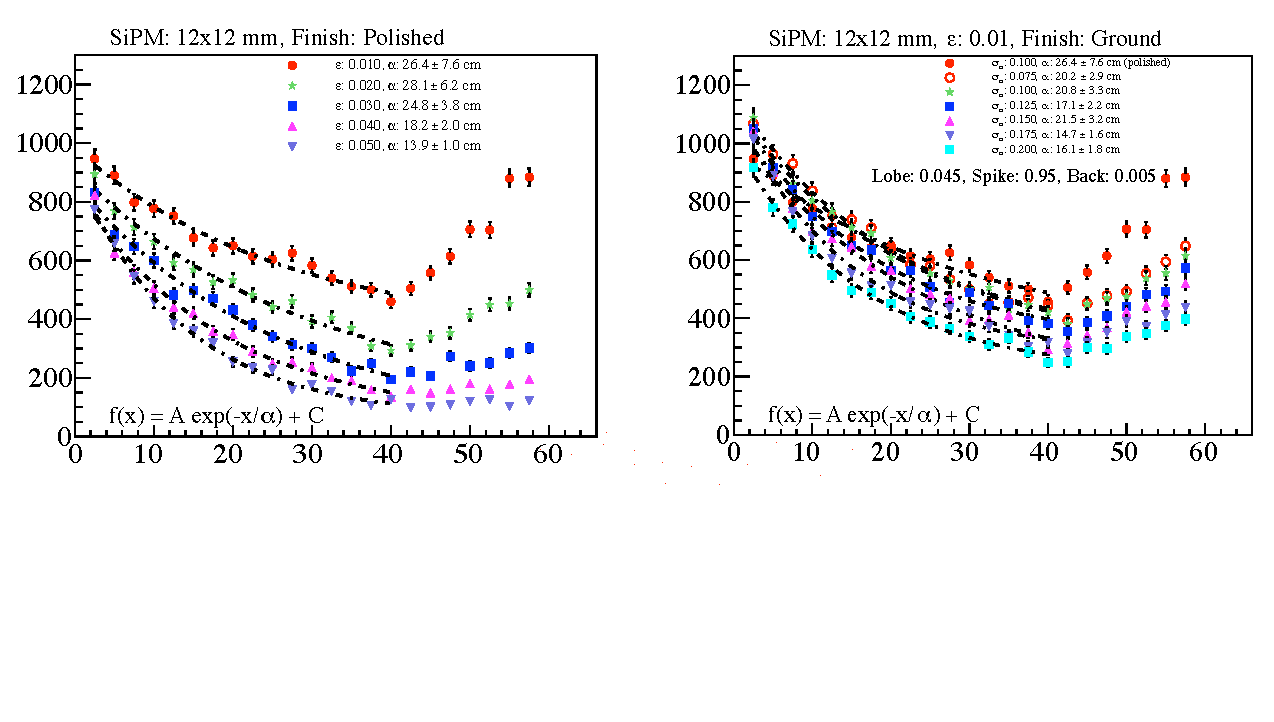
\includegraphics[width=1.0\columnwidth]{simulation/figs/transm_eff_vs_sig_alpha}
	\caption{UNIFIED Model results.  Left: polished model while varying the transmission efficiency.  Right: ground model with varying $\sigma_{\alpha}$ which characterizes the standard deviation of the surfaces micro-facet orientation.}
	\label{fig:transm_eff_vs_sig_alpha}
	\end{figure}
It is clear that if the transmission efficiency is increased while assuming a polished surface, the amount of light collected in the SiPM also increases as illustrated in Fig.~\ref{fig:transm_eff_vs_sig_alpha}.  Similarly, as the number of micro-facet orientations increase, meaning a more coarsely ground surface, the amount of light collection in the SiPM decreases.  Moreover, in the instances where the surface quality of the machined scintillators are good, the phenomenon of light increase in the nose region as the source moves further from the readout detector is observed.

 %WB suggestions
\section{Misalignment Studies} \label{sec:misalign}

In order to protect both the active area of the SiPMs and the scintillator surface at the upstream end, a small air gap was necessary between these two surfaces.  Similarly, during assembly the scintillator paddles were also shimmed radially such that the top edge of the scintillator was level with the top edge of the active area of the SiPM thereby maximizing light collection.  In this section we discuss the relative alignment of a machined scintillator paddle and a SiPM readout detector array and its effects on light collection and time resolution,

\subsection{Experimental Set-up} \label{sec:misalign_setup}
% WB this needs to be shortened and summarized. You can make references to your thesis for all the details.
% EP done.

A custom fabricated test stand, further discussed in Sec.~\ref{sec:fab_test}, and a polished scintillator machined to the nominal ST geometry, were utilized for the misalignment studies.  The readout SiPM sat atop a Newport MT-XYZ (MT) compact dovetail XYZ linear translation stage\cite{newport_mt_xyz} with three fine adjustment screws consisting of 80 threads per inch.  Each knob for the three axes provides a translation of $318\ \mathrm{\mu m}$ per rotation.  For each location of the SiPM, the source and trigger PMT were located $\mathrm{24.5~cm}$ downstream from the readout end. 

%To study the effects of the various horizontal (translations along the $z-axis$) coupling distances, the relative position of the active area of the SiPM and the top edge of the scintillator paddle, or vertical (translations along the $y-ais$) alignment, was required to be known prior too.

Utilizing an Edmund Optics complementary metal oxide semiconductor (CMOS) camera, the vertical alignment and horizontal alignment (coupling distance) of the active area of the SiPM and scintillator were measured with $25~\mathrm{\mu m}$ accuracy.
% WB make this schematical, the photos are no clear.
% EP done.
	\begin{figure}[!htb]
		\centering
		%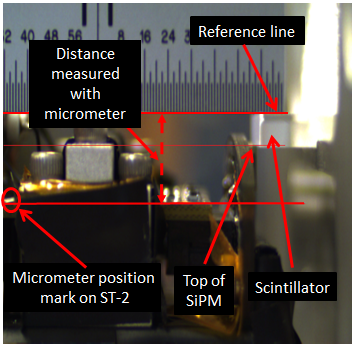
\includegraphics[width=0.8\columnwidth]{misalignment/figs/sipm_va_optics}
		%\caption{Vertical alignment optics set-up.  The reference line corresponds to the top surface of the scintillator, while the micrometer position on the ST2 is clearly marked so that the absolute difference could be measured both optically and manually with a micrometer.}
		%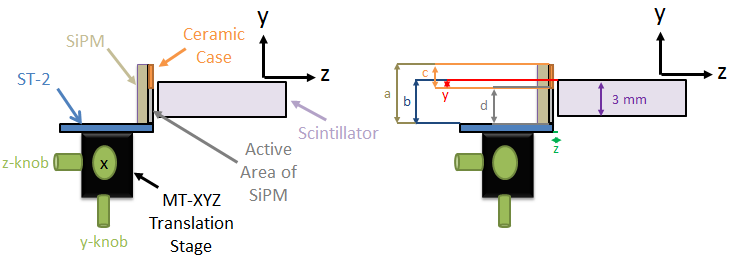
\includegraphics[width=1.0\columnwidth]{misalignment/figs/sipm_va_optics_schematic}
		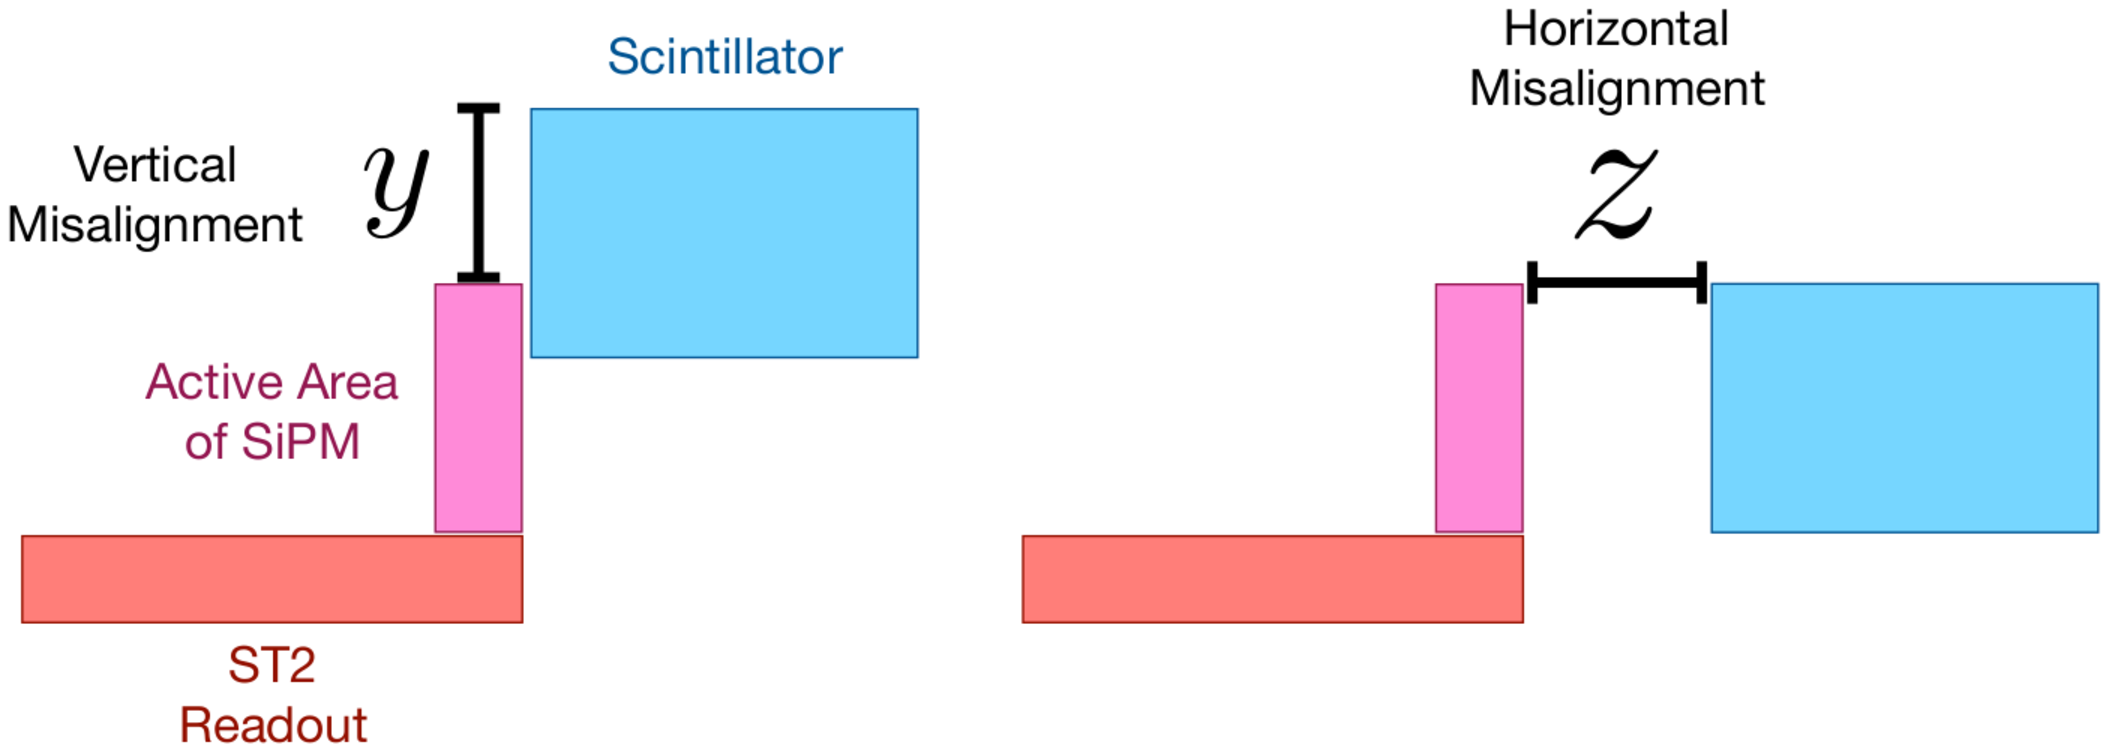
\includegraphics[width=1.0\columnwidth]{misalignment/figs/st_misalignment}
		\caption{Optics setup for misalignment studies.  Left: SiPM \&
		scintillator vertical misalignment. Right: SiPM \&
		scintillator horizontal misalignment}
		\label{fig:sipm_va_optics}
	\end{figure}
A micrometer, with $25~\mathrm{\mu m}$ resolution, was utilized in order to cross check the optical measurements and to provide absolute measurements of fixed distances in the experimental set-up. Further details of the experimental set-up are discussed in Ref.~\cite{pooser16}.

\subsection{Vertical Alignment of SiPM \& Scintillator}
\label{sec:misalign_vert}

% WB make the text shorter, basically just describe the result an compare to simulations. 
% EP done.
% WB The scales in Fig. 19 and 18 should be similar in order to compare simulation to measurement.
% EP the scales cannot be made similar since the simulation data no longer exists.

In order to measure the time resolution at various vertical alignment configurations, the scintillator remained fixed while the SiPM scanned across the upstream end of the scintillator as can be seen in the left of Fig.~\ref{fig:sipm_va_optics}. The coupling distance between the active area of the SiPM and scintillator ($z$) remained at a constant distance of $\mathrm{100\ \mu m}$ and was monitored closely during the vertical alignment scan.  We have defined that at $y = 0$ the SiPM and scintillator are aligned vertically.  %The SiPM was lowered to the minimum location governed by the range of the MT translation stage which was measured to be $y = \mathrm{-4~mm}$.  

%``Coarse'' measurements were then taken at half turn intervals $(159\ \mathrm{\mu m})$ until the maximum height of the MT translation stage was reached which was approximately $y = +4\ \mathrm{mm}$.  In order to conduct ``precise'' measurements the SiPM was lowered to $y = \mathrm{-1~mm}$ and then the translation stage was moved in quarter turn intervals $(79.5\ \mathrm{\mu m})$ until it reached $y = \mathrm{+1~mm}$.  The results of these measurements can be seen in Fig. \ref{fig:sipm_va_coarse}.
``Coarse'' measurements were then taken at half turn intervals $(159\ \mathrm{\mu m})$ while ``precise'' measurements were taken in quarter turn intervals $(79.5\ \mathrm{\mu m})$.  The results of these measurements can be seen in Fig. \ref{fig:sipm_va}.
%	\begin{figure}[!htb]
%		\centering
%		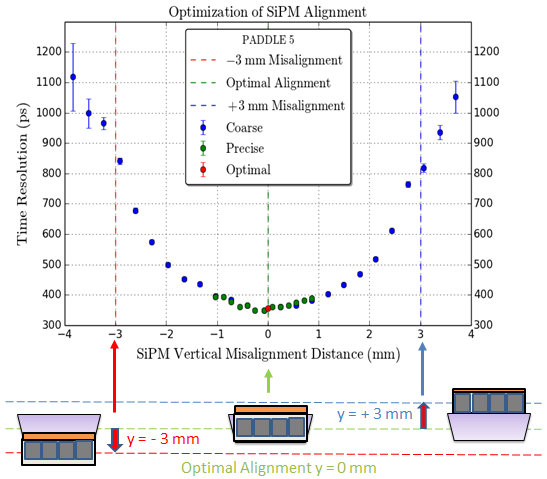
\includegraphics[width=1.0\columnwidth]{misalignment/figs/sipm_va_coarse}
%		\caption{Vertical misalignment results.  The minimum time resolution obtained was approximately 350 ps which was expected.  Once the SiPM exceeded $y = \pm 3\ mm$, no active area of the SiPM was directly coupled to the face of the scintillator.}
%		\label{fig:sipm_va_coarse}
%	\end{figure}
	\begin{figure}[!htb]
	\centering
	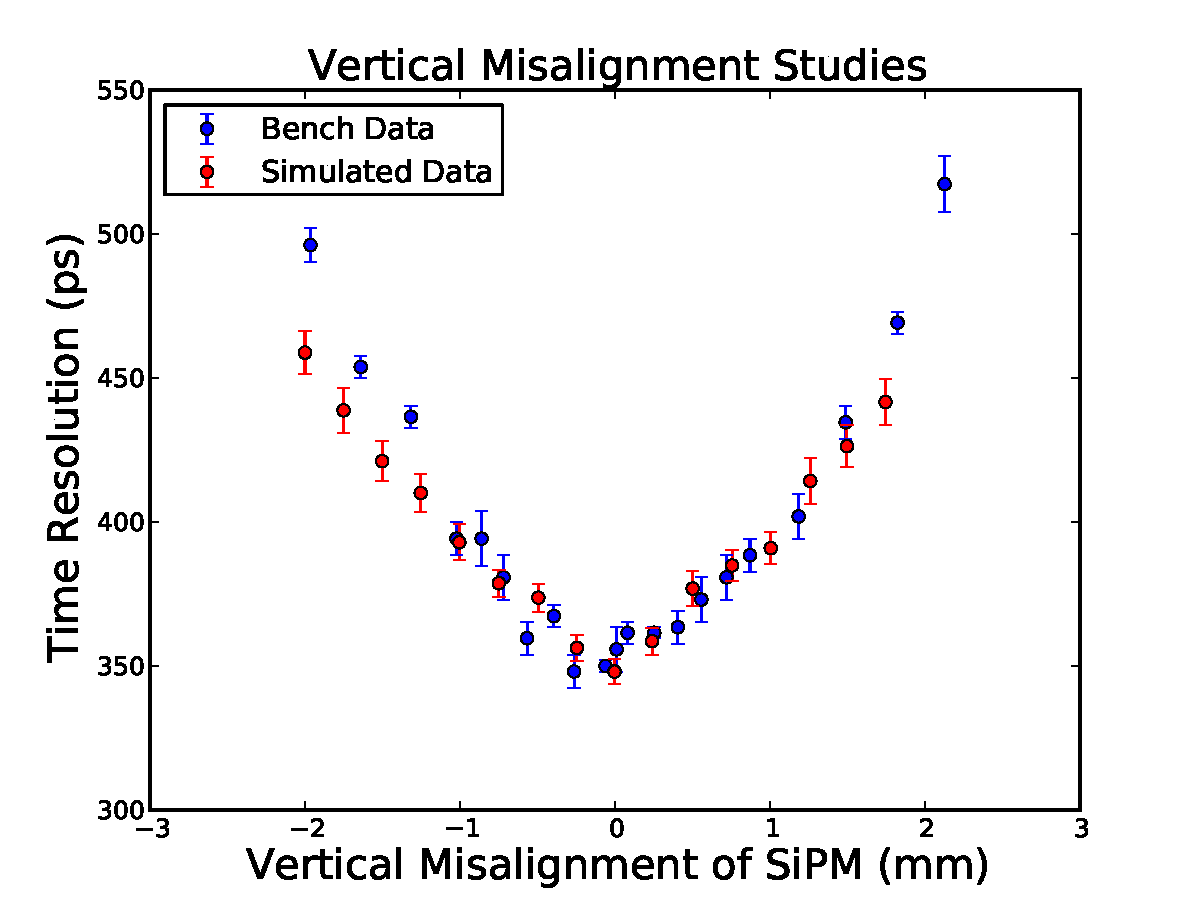
\includegraphics[width=1.0\columnwidth]{misalignment/figs/vert_ma}
	\caption{Vertical misalignment results.  The minimum time resolution obtained was approximately 350 ps which was expected.  Once the SiPM exceeded $y = \pm 3\ mm$, no active area of the SiPM was directly coupled to the face of the scintillator.}
	\label{fig:sipm_va}
\end{figure}
%For each distinct location of the SiPM, the distance traversed was verified by a manual measurement made with a micrometer with $25\ \mu m$ precision.
%From the vertical misalignment studies it is clear that there is no significant variation of time resolution within a $\pm 300\ \mathrm{\mu m}$ range of the optimal alignment.
The results indicate that there is no significant variation of time resolution within a $\pm 300\ \mathrm{\mu m}$ range of the optimal alignment.  

Vertical misalignments were also simulated in a manner similar to what was discussed in section \ref{sec:sim_mach} and the results are seen in Fig. \ref{fig:sipm_va}.
%	\begin{figure}[!htb]
%		\centering
%		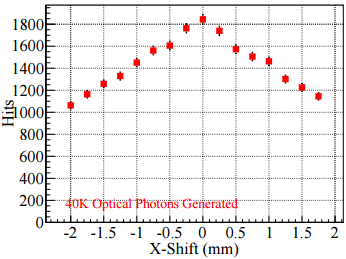
\includegraphics[width=0.8\columnwidth]{misalignment/figs/vertical_sim}
%		\caption{Vertical alignment simulation studies \cite{puneet_sim_talk}.}
%		\label{fig:vertical_sim}
%	\end{figure}
The GEANT4 simulations indicate that the acceptable range of vertical misalignment is approximately $\pm 250\ \mathrm{\mu m}$ \cite{puneet_sim_talk} which is consistent with what was measured on the bench.

\subsection{Coupling Distance of SiPM \& Scintillator}

With the vertical alignment between the scintillator and SiPM optimized, the effects of varying the coupling distance were also studied.  Using an identical set-up as was described in section \ref{sec:misalign_vert} the coupling distance, and resulting time resolutions, were measured at various locations along $z$ illustrated in Fig.~\ref{fig:sipm_va_optics}.  While the coupling distance was varied, the vertical alignment was kept constant at the optimal location and was monitored both optically and manually with a micrometer.
% WB skip thiso figure  
% EP done.
%	\begin{figure}[!htb]
%		\centering
%		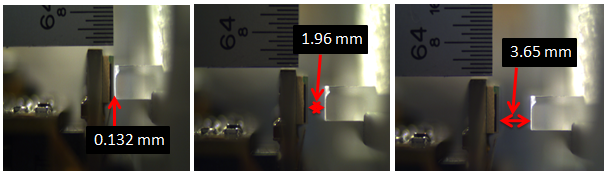
\includegraphics[width=1.0\columnwidth]{misalignment/figs/sipm_coupling_optics}
%		\caption{Various coupling distances as measured with the CMOS camera.  The high degree of precision is clearly visible.}
%		\label{fig:sipm_coupling_optics}
%	\end{figure}

%The SiPM was moved \textit{via} the MT translation stage along the $z-axis$.  We defined $z = 0$ to be the instance when the active area of the SiPM was flush against the face of the machined scintillator paddle.  In the coupling region $z < 1\ \mathrm{mm}$ the SiPM was receded from the face of the SiPM in 1/4 turn intervals ($79.5\ \mathrm{\mu m}$).  For $\mathrm{1\ mm < z < 2\ mm}$, the SiPM was receded from the face of the SiPM in 1/2 turn intervals ($159\ \mathrm{\mu m}$), and for $\mathrm{2\ mm < z < 4\ mm}$ data were collected in 1 turn intervals ($\mathrm{318\ \mu m}$) with the results being illustrated in Fig. \ref{fig:sipm_coupling_coarse}.
The SiPM was moved \textit{via} the MT translation stage along the $z-axis$.  We defined $z = 0$ to be the instance when the active area of the SiPM was flush against the face of the machined scintillator paddle.  Further details regarding the three coupling intervals shown in Fig. \ref{fig:sipm_coupling} are discussed further in Ref.~\cite{pooser16}.  The results of this study is illustrated in Fig. \ref{fig:sipm_coupling}.
%	\begin{figure}[!htb]
%		\centering
%		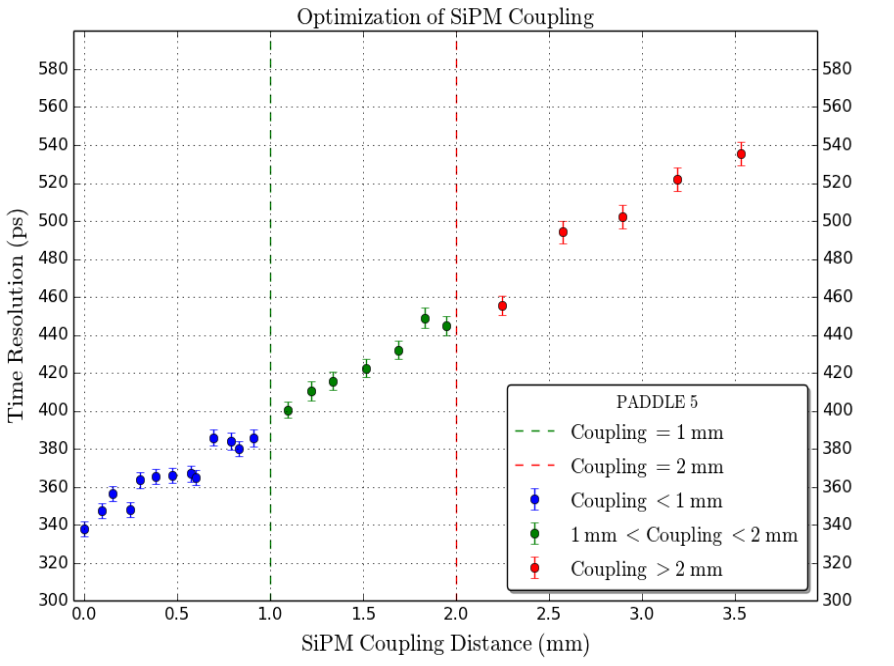
\includegraphics[width=0.83\columnwidth]{misalignment/figs/sipm_coupling_coarse}
%		\caption{Coupling distance studies.  It is useful to note that at a coupling distance of $\mathrm{251\ \mu m}$ the time resolution was identical to what was measured in Fig. \ref{fig:sipm_va} while conducting the vertical alignment studies.}
%		\label{fig:sipm_coupling_coarse}
%	\end{figure}
	\begin{figure}[!htb]
	\centering
	\includegraphics[width=0.83\columnwidth]{misalignment/figs/hori_ma}
	\caption{Coupling distance studies.  It is useful to note that at a coupling distance of $\mathrm{251\ \mu m}$ the time resolution was identical to what was measured in Fig. \ref{fig:sipm_va} while conducting the vertical alignment studies.}
	\label{fig:sipm_coupling}
	\end{figure}

It is clear from the data that the optimal coupling range was $\mathrm{50\ \mu m < z < 350\ \mu m}$ and there was no significant reduction in time resolution performance over a $\mathrm{0\ \mu m < z < 600\ \mu m}$ range.  Similarly, the simulation results seen in Fig.~\ref{fig:sipm_coupling} also indicate that there is no significant reduction in light collection in the $\mathrm{0\ \mu m < z < 600\ \mu m}$ range \cite{puneet_sim_talk}.
%	\begin{figure}[!htb]
%		\centering
%		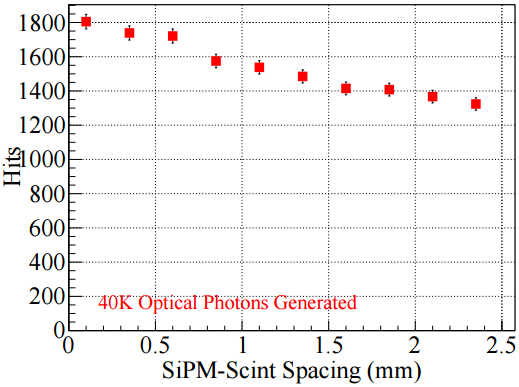
\includegraphics[width=0.8\columnwidth]{misalignment/figs/spacing_sim}
%		\caption{Coupling distance simulations. Simulations indicated that the optimal coupling distance is in the $50\ \mu m < z < 350\ \mu m$ range.}
%		\label{fig:spacing_sim}
%	\end{figure} %WB suggestions
\section{Fabrication} \label{sec:fab}

In order to successfully identify the 2 ns electron beam bunch structure delivered by the CEBAF to within 99\% accuracy, the \gx{} Start Counter time resolution is required to be $<350\ \mathrm{ps}$.  In the following section the details of polishing and characterizing machined scintillators, as well as the construction of the Start Counter are discussed.

\subsection{Polishing Machined Scintillators} \label{sec:fab_polish}

The surfaces of the machined scintillators incurred a plethora of surface defects and chemical contaminants known to harm scintillator surfaces while undergoing edge polishing at McNeil Enterprises.  Therefore, in an effort to recover the performance capabilities, polishing was required.

Prior to polishing the machined scintillators, a coarse measurement of the paddles performance was conducted.
% to understand the magnitude of damage the paddles had incurred, relative to prototypes, as a result of mishandling.  
The time resolution and light output was measured at three precise locations along the length of the scintillators. One measurement was taken in the middle of the straight section, one in the middle of the bend, and one at the tip of the nose. 

Figure~\ref{fig:Initial_Paddle_Prop_UW} illustrates the erratic fluctuation and poor performance that existed from paddle to paddle prior to polishing. 
	\begin{figure}[!htb]
		\centering
		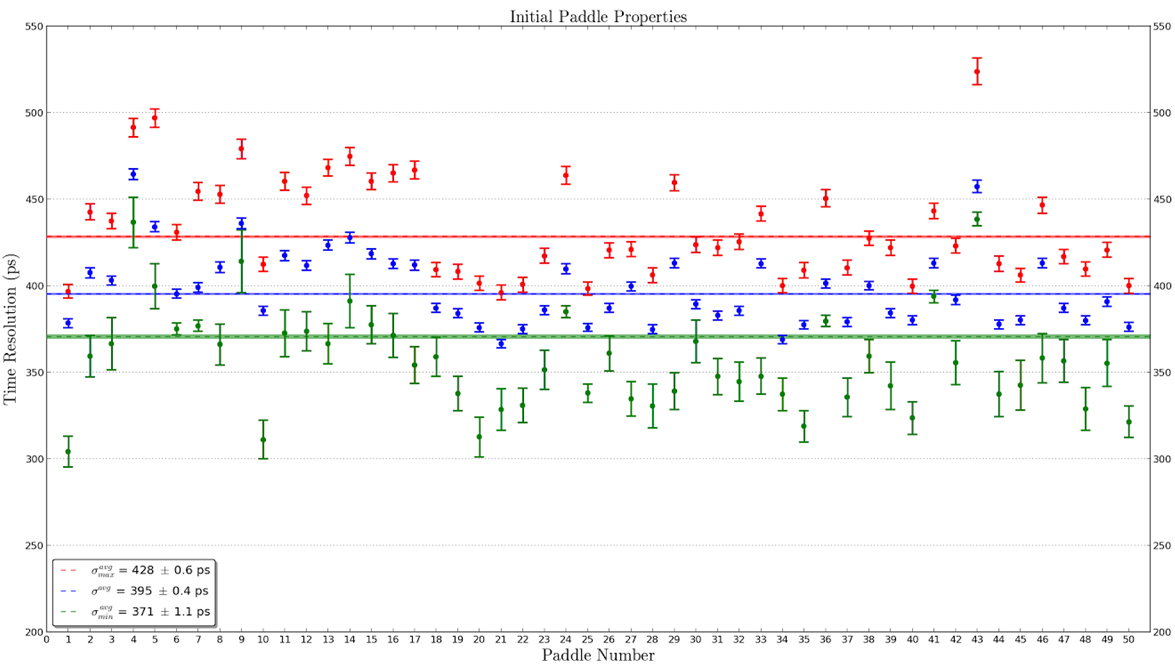
\includegraphics[width=1.0\columnwidth]{fabrication/figs/Initial_Paddle_Prop_UW}
		\caption{Coarse time resolution measurements prior to polishing. Paddle number is on the x-axis and time resolution in ns is on the y-axis. The red points are the resolutions in the bend region, the blue points are the weighted average of the three measurements, and the green points are the resolutions at the tip of the nose.  The horizontal lines are the weighted averages of the individual measurements.}
		\label{fig:Initial_Paddle_Prop_UW}
	\end{figure}
On average the 50 paddles did not meet the design resolution of 350 ps.

To polish the machined scintillator surfaces, Buehler Micropolish II deagglomerated $\mathrm{0.3\ \mu m}$ alumina suspension was utilized \cite{buehler}.  The polishing suspension was diluted with a 5:1 ratio of de-ionized $\mathrm{H_{2}O}$ to alumina and applied to a cold, wet $6'' \times 0.5''$ Caswell Canton flannel buffing wheel \cite{caswell} operated at $\mathrm{<1500~RPMs}$. All surfaces of the scintillators were carefully buffed until all large, uniform surface defects were removed. In order to eliminate small, localized surface defects hand polishing with a soft NOVUS premium Polish Mate microfilament cloth \cite{novus} and diluted polishing suspension was applied.  These polishing procedures made the scintillators void of virtually all scratches and surface defects.

Once the appropriate polishing procedures had been developed and implemented the surface quality was greatly improved as can be seen in Fig.~\ref{fig:polshing_effects} which illustrates the same scintillator paddle before and after polishing.
	\begin{figure}[!htb]
		\centering
		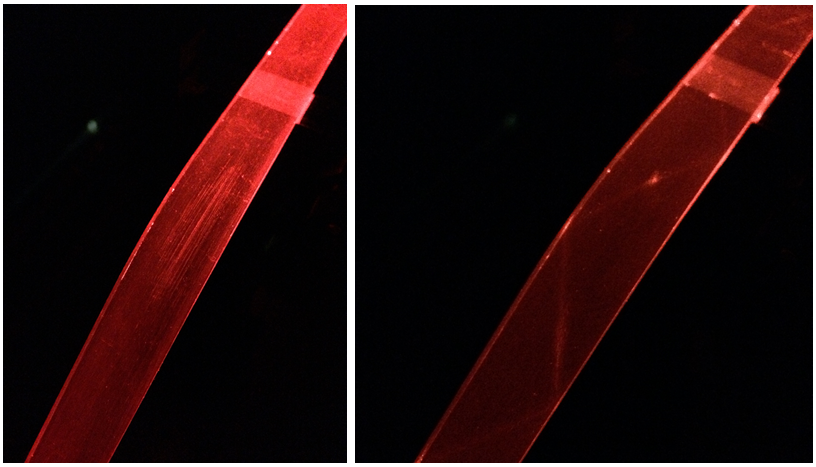
\includegraphics[width=1.0\columnwidth]{fabrication/figs/polshing_effects}
		\caption{Effects of polishing scintillators. Left: non-diffuse laser incident on an edge, before polishing, at the upstream end of the straight section. Right: non-diffuse laser incident on the same edge, after polishing, at the upstream end of the straight section.}
		\label{fig:polshing_effects}
	\end{figure}
A red laser beam was shone into the scintillator medium from the upstream end aimed at one edge so that the total internal reflection towards the tip of the nose was visible.  The unpolished scintillator had such poor surface quality that the reflections in the bend region could not be seen due to the multiple scattering of light at the scintillator boundaries.  However, the reflections in the polished scintillator can clearly be seen traversing down through the nose region.

Once the scintillators were polished, their performance was remeasured so that a quantitative measure of the polishing effects were understood.  The measurements were performed in an identical manner outlined above and the pre-polished results were illustrated in Fig.~\ref{fig:Initial_Paddle_Prop_UW}. As expected, the time resolutions were improved as seen in Fig.~\ref{fig:Polished_Paddle_Prop_UW}.
	\begin{figure}[!htb]
		\centering
		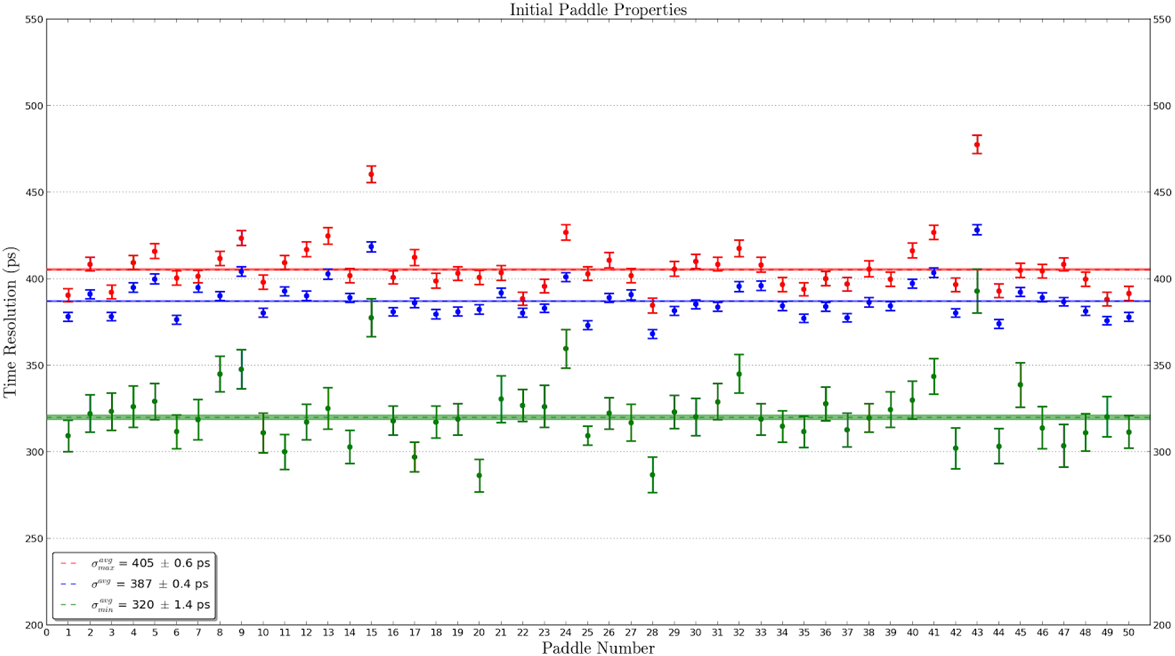
\includegraphics[width=1.0\columnwidth]{fabrication/figs/Polished_Paddle_Prop_UW}
		\caption{Coarse time resolution measurements after polishing. The details are identical to Fig.~\ref{fig:Initial_Paddle_Prop_UW}}
		\label{fig:Polished_Paddle_Prop_UW}
	\end{figure}
On average, at the tip of the nose, the scintillators exhibited a $\approx15\%$ improvement in time resolution.  Moreover, there was a substantial reduction in erratic fluctuations in performance.

\subsection{Testing} \label{sec:fab_test}

The polished scintillators were tested in order to determine their light output and time resolution properties.  They were measured in an identical and reproducible manner utilizing a custom fabricated test stand shown in Fig.~\ref{fig:test_stand_model}. 
	\begin{figure}[!htb]
		\centering
		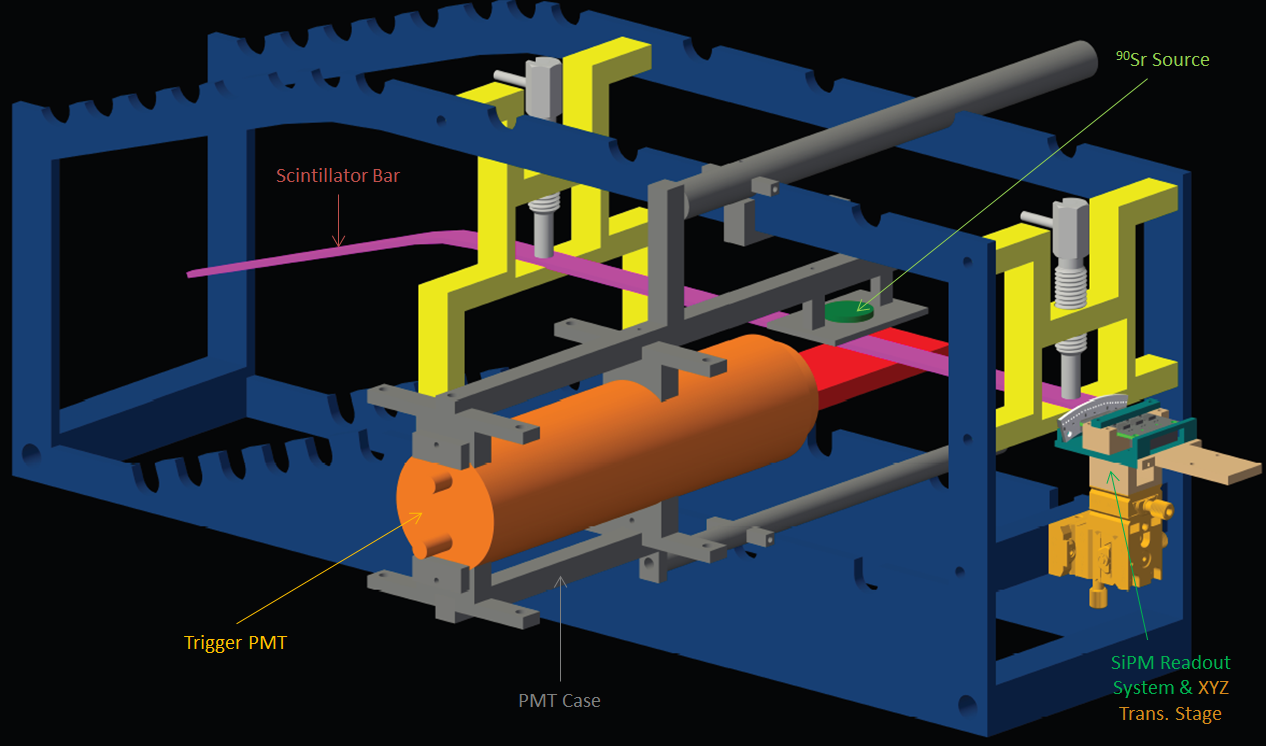
\includegraphics[width=1.0\columnwidth]{fabrication/figs/test_stand_model}
		\caption{CAD Drawing of custom test stand.}
		\label{fig:test_stand_model}
	\end{figure}
The test stand facilitated the precise measurement of the aforementioned scintillator properties at 12 well-defined locations along the length of the scintillator paddles.  Specifically 4 locations in the straight section, 3 in the bend, and 5 in the nose were tested.  

The measurements were conducted with a collimated $\mathrm{^{90}Sr}$ source oriented orthogonal to the wide flat surface of the scintillators.  The $\mathrm{^{90}Sr}$ source provided minimum ionizing electrons ranging in energy from $\mathrm{0.5-2.3~MeV}$ \textit{via} beta-decay \cite{nndc_sr90}\cite{nndc_y90}.  A trigger photo-multiplier tube (PMT) was placed underneath the scintillator on the opposite side of the $\mathrm{^{90}Sr}$ source and provided the TDC start time and ADC gate.  A SiPM detector array identical to the ones installed in the final ST assembly, was used for readout.  

%The signals from the SiPM and the trigger PMT were then recorded in our data acquisition computer configured with the CEBAF on-line data acquisition (CODA) software.  The signal processing electronics diagram is illustrated in Fig.~\ref{fig:nimelectronicsdiagram}.
%% WB I am not sure we need this here as it is pretty standard
%% EP done.
%	\begin{figure}[!htb]
%		\centering
%		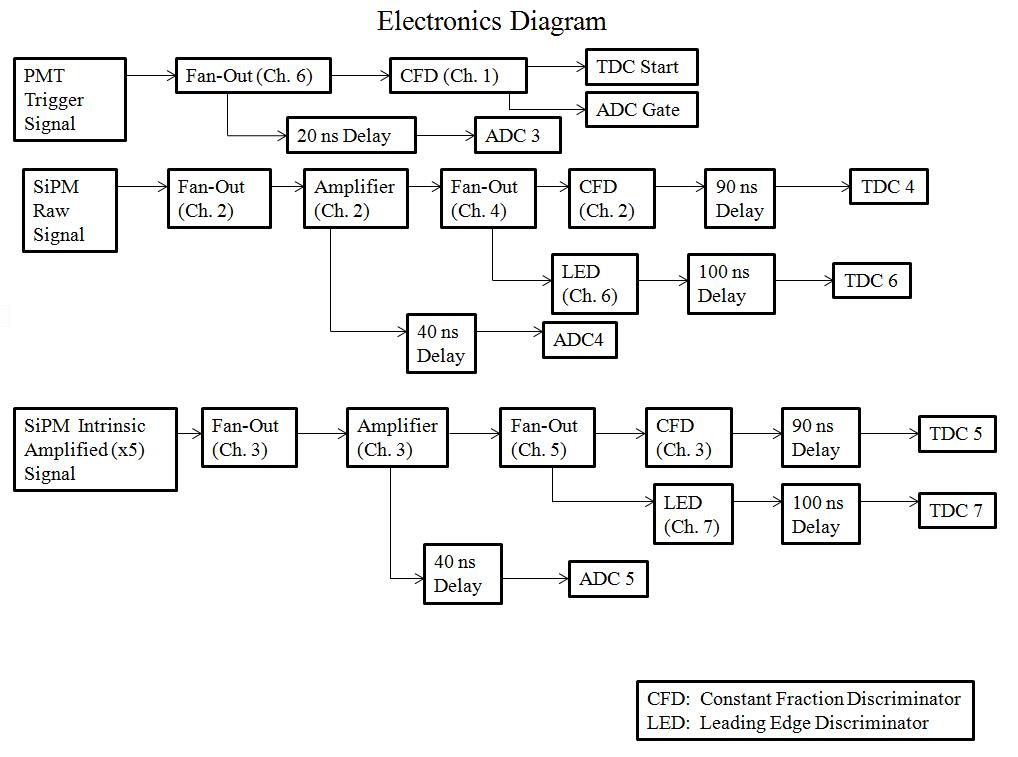
\includegraphics[width=1.0\columnwidth]{fabrication/figs/nim_electronics_diagram}
%		\caption{Electronics diagram for testing machined scintillators.}
%		\label{fig:nimelectronicsdiagram}
%	\end{figure}
The signals from the SiPM and the trigger PMT were then recorded in our data acquisition computer configured with the CEBAF on-line data acquisition (CODA) software.  10,000 event triggers and associated data were collected at each of the locations along the scintillator path.  Subsequently, the ADC and TDC data were analyzed to measure the light output and time resolutions respectively of the whole lot of polished machined scintillators.  

Once the 30 machined scintillator paddles which exhibited the best time resolution and light output properties from the lot of 50 were selected, they were carefully wrapped in Reynolds food grade aluminum foil.  The aluminum foil is $\mathrm{16.5~\mu m}$ thick and possesses good reflectivity properties.  Moreover, the aluminum foil protects the surfaces of the scintillators during both the testing and assembly processes.
  
The measured time resolutions for the 30 best scintillators, which comprise the ST, were found to be satisfactory and even well below design resolution in the nose region which is illustrated in Fig.~\ref{fig:time_res_comp_final_30}.
	\begin{figure}[!htb]
		\centering
		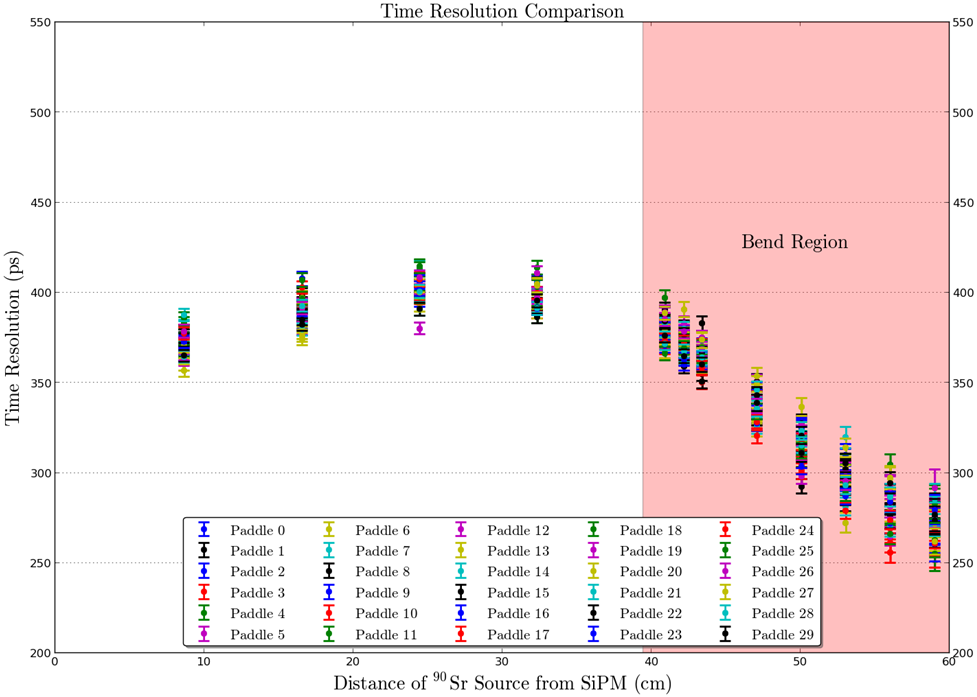
\includegraphics[width=1.0\columnwidth]{fabrication/figs/time_res_comp_final_30}
		\caption{Time resolution of 30 the best scintillator paddles.  The time resolution performance of the selected scintillators is remarkably similar while illustrating a spread of $\approx 50\ ps$ in the nose region.}
		\label{fig:time_res_comp_final_30}
	\end{figure}

The unique geometry of the machined scintillator paddles exhibit a phenomenon of an increase in light collection in the nose region as the light source moves towards the tip at the downstream end.  It is hypothesized that the relatively poor time resolution in the straight section is due to a reflective smearing effect in which light is able to traverse from the straight section down to the tip of the nose, and then back up to the upstream end.

The average time resolution of the individual scintillators selected for the final ST assembly are shown in Fig.~\ref{fig:final_30_tr_wrapped}.
	\begin{figure}[!htb]
		\centering
		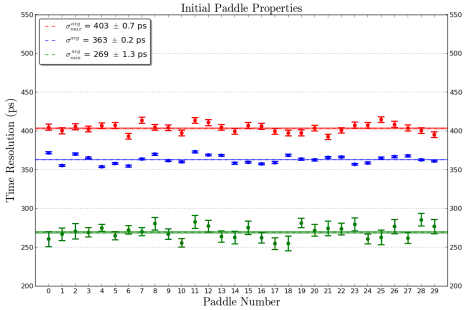
\includegraphics[width=1.0\columnwidth]{fabrication//figs/final_30_tr_wrapped}
		\caption{Average time resolution of 30 best scintillator paddles.  The red data points correspond to the maximum time resolution obtained in all 12 data points. The blue data points are the weighted average of all 12 data points.  The green data points indicate the minimum time resolution obtained in all 12 data points.}
		\label{fig:final_30_tr_wrapped}
	\end{figure}

\subsection{Assembly} \label{sec:fab_ass}

% WB we need a better drawing here
% EP I do not have one
In order to assemble the ST an assembly jig, illustrated in Fig~\ref{fig:ajcaddrawing}, was fabricated.  
	\begin{figure}[!htb]
		\centering
		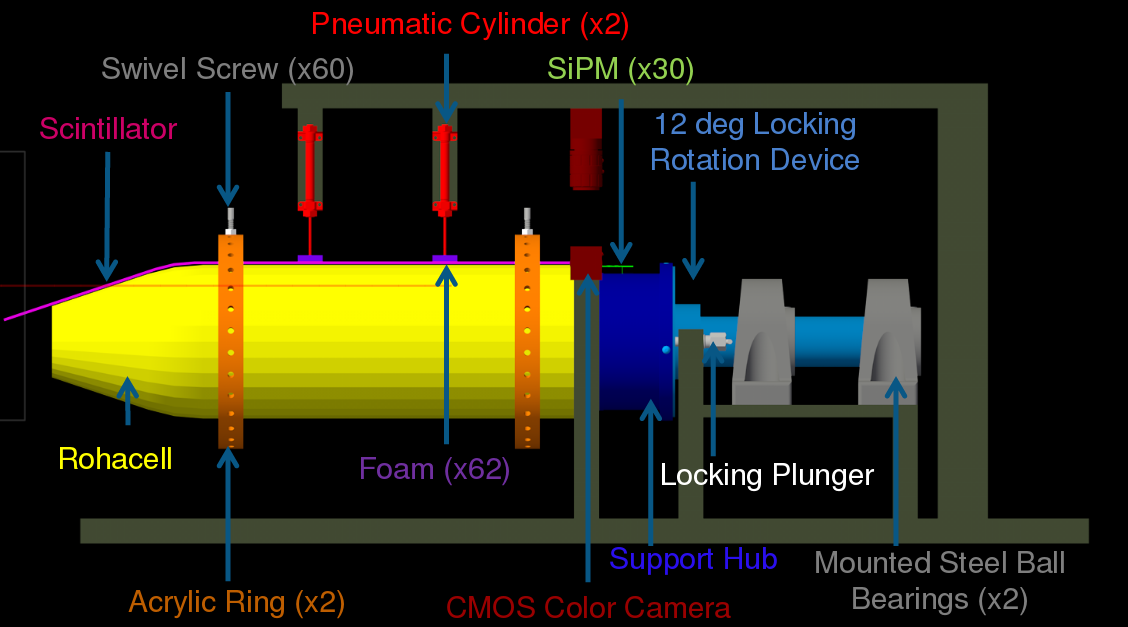
\includegraphics[width=1.0\columnwidth]{fabrication/figs/aj_cad_drawing}
		\caption{CAD drawing of the ST assembly jig.}
		\label{fig:ajcaddrawing}
	\end{figure}
% references to the drawing are needed here suchas :
% consisted of a rotating cylindrical mounting bracket(a) rigidly attached to a 2'' diameter shaft (b) etc. ...
% EP done.
The jig consisted of a rotating cylindrical mounting bracket (light-blue) rigidly attached to a 2'' diameter shaft (light-blue) housed in two cast iron mounted steel ball bearings (gray).  The rotating bracket was engineered such that it was free to rotate unless engaged by a spring loaded locking plunger (light-gray) which would cause the assembly jig to move in discretized $12^{\circ}$ intervals.  This provided the ability to orient paddles (magenta) parallel to the table top so that alignment and coupling could be performed reliably and reproducibly.

While mounted to the assembly jig, the upstream chassis (dark-blue) and Rohacell (yellow) was attached to the rotating bracket.  A vertical bar (dark-green) running parallel to the table above the Rohacell served as a mount for the pneumatic cylinders (red) so that the scintillators could be held firmly in place during installation.  Furthermore, it provided a surface in which a portable flex arm could hold a machine vision camera (dark-red) to monitor the coupling of the scintillators and SiPMs.

A pressurized gas system was implemented to provide manual control of the two pneumatic cylinders with soft, semi-dense rubber feet (purple) attached to the ends.  The rubber feet would hold the scintillator being installed firmly in place by activating two switches which controlled each pneumatic cylinder independently \textit{via} bi-directional solenoids connected in a 5 psi nitrogen gas system.

Two free floating acrylic rings (orange), with 30 tapped holes $12^{\circ}$ apart, were fabricated so as to firmly hold the scintillator paddles in place during assembly. 
%	\begin{figure}[!htb]
%		\centering
%		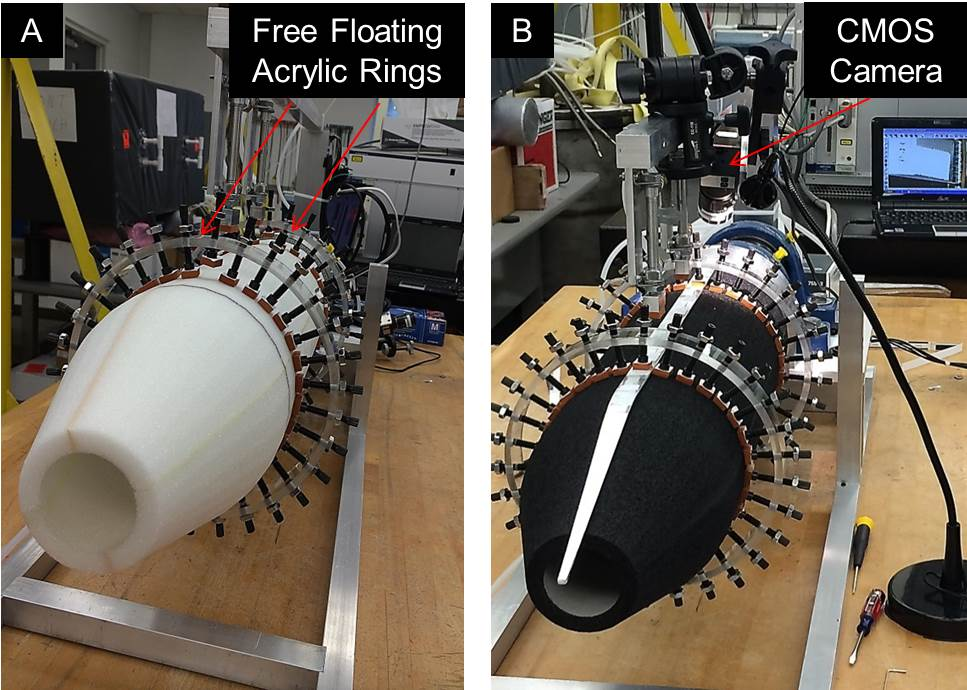
\includegraphics[width=1.0\columnwidth]{fabrication/figs/st_assembly}
%		\caption{Free floating acrylic rings.  Left: Rohacell prior to being painted with black latex paint. Each free floating ring is supported by 30 swivel pad screws. Right: Rohacell after being painted black.  One wrapped scintillator paddled is being held firmly in place by two swivel pad screws.}
%		\label{fig:free_floating_rings}
%	\end{figure}
Each tapped hole housed a $10^{\circ}$ swivel pad thumb screw (light gray) which had silicone foam foot $(0.25 \times 0.25\ \mathrm{in^{2}})$ adhered to it in order to provide a soft barrier between swivel pad and the scintillator surface. 

The camera, seen in Fig.~\ref{fig:aligning_st1_to_hub}, and its associated software were utilized to both measure and control the scintillator/SiPM coupling distances as well as the shimming heights with a precision of $\mathrm{< 10\ \mu m}$ in real time. 
	\begin{figure}[!htb]
		\centering
		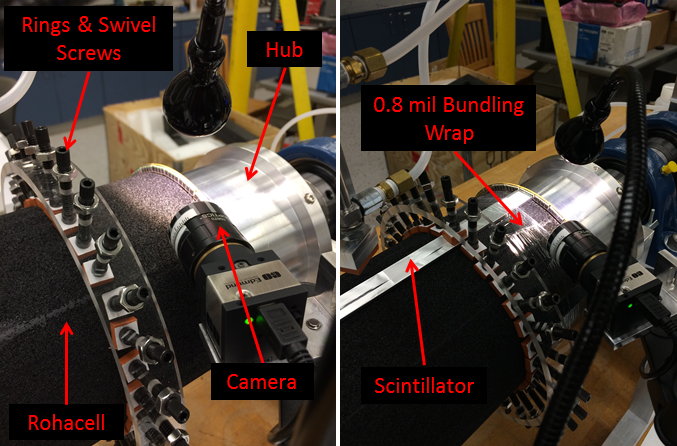
\includegraphics[width=1.0\columnwidth]{fabrication/figs/aligning_st1_to_hub}
		\caption{Aligning ST1 to support hub.  Left: CMOS camera and lamp prepared to monitor ST1 positioning.  Right: Reference scintillator wrapped to Rohacell during ST1 alignment.}
		\label{fig:aligning_st1_to_hub}
	\end{figure}
The camera was calibrated such that at various magnification settings the distance to pixel ratio was known.  The 10 ST1 boards were mounted to the pre-fixed tapped holes along the lip of the upstream support hub.  Black 1 mm spacers were installed between the ST1 PCB and the support hub to avoid any possibility of the electrical contact between the two.  The position of the ST1 was adjusted such that the distance between the top edge of the scintillator and the top edge of the active area of the SiPM was offset by 30 mils ($\mathrm{762\ \mu m}$).  %The offset was measured with the CMOS camera. 

% you do not provide detailed mounting instructions here just the results and parameters

%Each scintillator paddle was carefully installed such that a quantitative measure of the coupling distance and amount of radial shimming required was determined with a high degree of precision and is illustrated in Fig.~\ref{fig:aligning_st1_to_hub}. 

On average each paddle required 30~mils of Kapton polyimide heavy duty film (type HN, $\rho = 1.42\ \mathrm{g/cm^{3}}$) radial shimming.  Moreover, the scintillators were coupled to the SiPM's at a distance of $\mathrm{<\ 200\ \mu m}$.  More details regarding the assembly process are discussed in Ref.~\cite{pooser16}.

%The paddle being installed was carefully positioned such that the upstream end was located approximately a millimeter away (downstream) from the active area of the SiPM and were held in place as seen in Fig.~\ref{fig:aligning_st1_to_hub}. 
%A piece of 0.8~mil bundling wrap was wrapped firmly around the scintillator and the Rohacell structure as seen in Fig.~\ref{fig:aligning_st1_to_hub}. 
% WB pictures can be reduced here
% EP done.

%The distance between the top edge of the scintillator and the top edge of the active area of the SiPM was then measured in order to determine the amount of shimming necessary for radial alignment as illustrated in Fig.~\ref{fig:shimming_effects}. 
%	\begin{figure}[!htb]
%		\centering
%		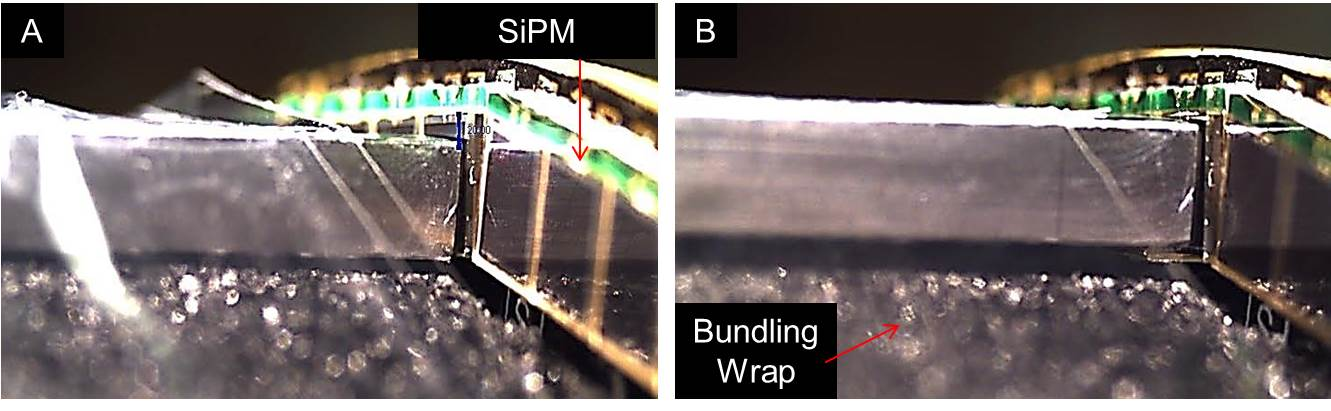
\includegraphics[width=1.0\columnwidth]{fabrication/figs/st_va}
%		\caption[Shimming effects]{Shimming effects.  Left: Before and Right: after shimming.}
%		\label{fig:shimming_effects}
%	\end{figure}
%Three different thickness's (5, 10, 20 mil) of Kapton polyimide heavy duty film (type HN, $\rho = 1.42\ \mathrm{g/cm^{3}}$) were cut into $\mathrm{0.5 \times 12\ in^{2}}$ strips and utilized for shimming the scintillators in the radial direction.  On average, each paddle required 30~mils of radial shimming.

%With the appropriate shimming in place, the paddle was carefully positioned such that the center of the upstream paddle was aligned with the center of the SIPM and the swivel screws were extended.  A piece of computer paper sandwiched between two pieces of Al foil ($\approx 150\ \mathrm{\mu m}$ thick) was then placed parallel to the active are of the SiPM and the paddle was then pressed firmly against the outer most piece of Al foil which is seen in Fig.~\ref{fig:sipm_coupling}.
% WB Pcitures are not necessary here may be a schematic drawing
%	\begin{figure}[!htb]
%		\centering
%		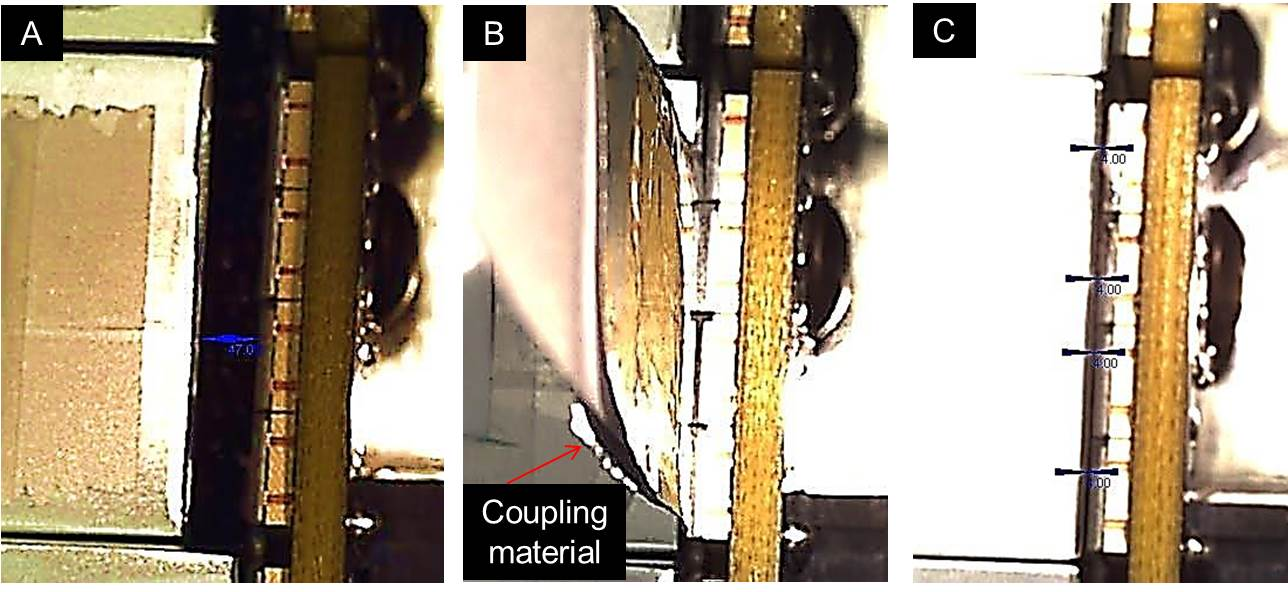
\includegraphics[width=1.0\columnwidth]{fabrication/figs/st_coupling}
%		\caption{Steps of coupling paddles to SiPM.  Left: Paddle prior to being coupled to SiPM.  Center:  Paddle pressed firmly against spacing material and SiPM.  Right: Paddle properly coupled to SiPM at a distance of $162\ \mu m$.}
%		\label{fig:sipm_coupling}
%	\end{figure}
%The piece of computer paper was carefully removed. Then, the Al foil pieces were removed individually so as to ensure no damage was incurred on the paddle surface or SiPM.  Utilizing this method provided a coupling distance $\mathrm{<\ 200\ \mu m}$.

In order to make the ST light tight, an inner cone of black Tedlar polyvinyl fluoride $\rho \approx 1.5\ \mathrm{g/cm^{3}}$ \cite{tedlar_pvf} was taped to the Rohacell as seen in Fig.~\ref{fig:light_tightening_cone}. 
\begin{figure}[!htb]
	\centering
	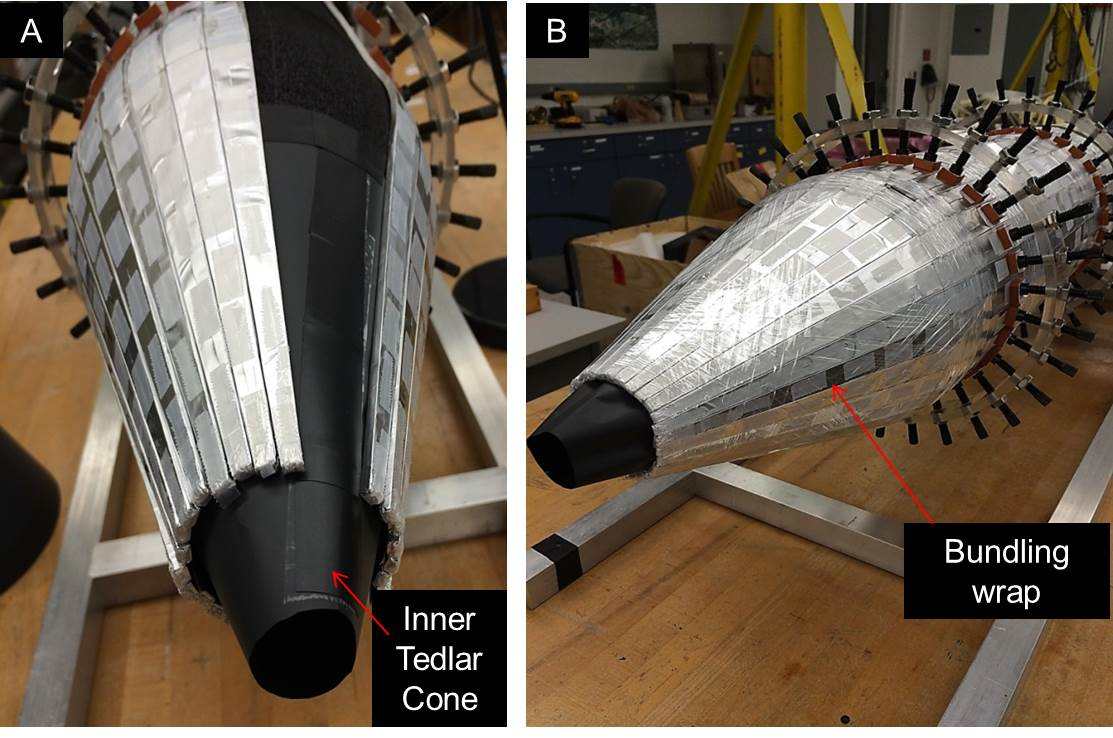
\includegraphics[width=1.0\columnwidth]{fabrication/figs/st_lt_ic_bw}
	\caption{Inner Tedlar cone.  Shown is before and after wrapping with bundling wrap.  The cone was specifically engineered to have the same dimensions of the Rohacell support structure to avoid crumpling of the light tightening material.}
	\label{fig:light_tightening_cone}
\end{figure}
A few gaps existed in the Rohacell at the glue joints, and were filled in with black RTV silicone caulking. Moreover, it was painted with black latex paint for light tightening purposes.  The support hub was also was wrapped with Tedlar and taped down with black electrical tape. The spacing between the ST1 PCBs along with the bottom side of the support hub, was filled with RTV black opaque silicone caulking.  Similarly, RTV silicone caulking was then applied to the inner edge of the collar which encompassed the ST1 PCBs at their our diameter.

In order to secure paddles to the Rohacell support structure the Start Counter was wrapped along its length using self-adhesive transparent bundling wrap (0.8 mil thick, 6 in wide) at six different locations perpendicular to the central axis of rotation. Four locations were wrapped along the straight section at equal distance $(\approx 8\ \mathrm{cm})$ from one another, one in the bend and one in the nose section.  Five layers of bundling wrap were applied to each section.% and the acrylic rings were removed as illustrated in Fig.~\ref{fig:st_iso_eel}.
% WB only one picture here but with indicators where the bundling wrap sits
%\begin{figure}[tbph]
%	\centering
%	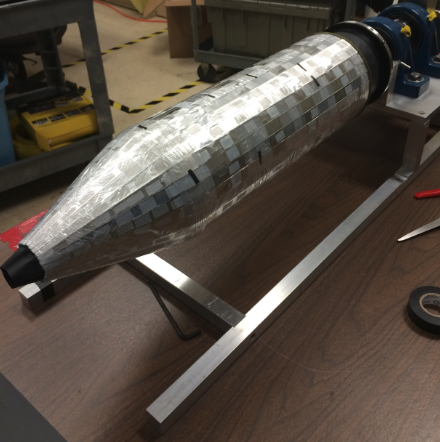
\includegraphics[width=0.8\columnwidth]{fabrication/figs/st_iso_eel}
%	\caption[Isometric view of assembled Start Counter]{Isometric view of assembled Start Counter. The pieces are black electrical tape which mark the ends of bundling wrap are clearly visible.}
%	\label{fig:st_iso_eel}
%\end{figure}

A cone of Tedlar was wrapped around the nose region and taped down with electrical tape as seen in Fig.~\ref{fig:light_tight_st}. 
\begin{figure}[!htb]
	\centering
	\includegraphics[width=1.0\columnwidth]{fabrication/figs/st_lt_v2}
	\caption{Light tight Start Counter mounted to the \gx{} $\mathrm{LH_{2}}$ target.}
	\label{fig:light_tight_st}
\end{figure}
The tips of the inner and outer cones in the nose region were then taped together with electrical tape and trimmed of excess material. Furthermore, a cylindrical piece of Tedlar was taped down at the bend region and to the collar covering the ST1 boards.  The fully assembled and cabled ST mounted to the commissioning target can be seen in Fig.~\ref{fig:light_tight_st}. 

%








% WB edit and suggestions
\section{Calibration} \label{sec:calib}

In this section the various calibration procedures taken in order to minimize the time resolution and enhance both the particle identification (PID) and time of flight (TOF) capabilities of the Start Counter are discussed.

\subsection{Time-Walk Correction} \label{sec:calib_tw}

The time-walk effect is a well understood consequence of leading edge discriminators (LED).  Analog signals of varying amplitudes crossing a fixed threshold, as determined by the discriminator threshold setting, will do so at varying times.

The time-walk effect is attributed to larger signals having faster rise times as compared to signals which have amplitudes close to the threshold setting, see Fig.~\ref{fig:time_walk_effect}.
\begin{figure}[!htb]
	\centering
	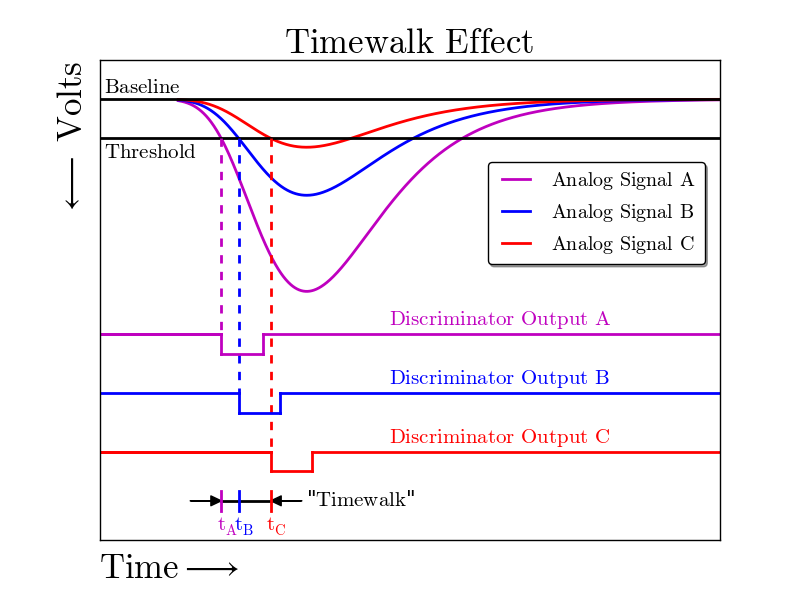
\includegraphics[width=1.0\columnwidth]{calibration/figs/time_walk_effect}
	\caption{Example of the time-walk effect. Three coincident analog signals A, B, \& C of varying amplitudes crossing a fixed threshold in a LED. The discriminator logic output signals vary in time relative to the amplitude of the incoming analog signal.  The signals shown above are simulated analog signals being fed into the LED's thus, they have negative polarity.}
	\label{fig:time_walk_effect}
\end{figure}
As seen in Fig.~\ref{fig:time_walk_effect}, signal A has a larger amplitude as compared to signals B \& C.  It is clear that the logic signal output from the discriminator ``\textit{walks about}'' in time, resulting in an undesirable increase in time resolution of the systems TDC channels.

The time to digital converter (TDC) times reported by the LEDs are subject to the time-walk effect and must be corrected for \textit{via} software so as to optimize the time resolution for each ST channel.  In order to correct the TDC times returned by the F1TDC's one must first acquire a reference time for each hit in the ST, for each event.   %WB edit and suggestions
\section{Performance} \label{sec:perform}

The Start Counter was installed in Hall-D just prior to the Fall 2014 \gx{} commissioning run.  It was not until the Spring 2015 commissioning run that enough statistics were obtained with an $\mathrm{LH_{2}}$ target to perform reliable calibrations.  With the aforementioned data set, the procedures to calibrate the detector and measure it's performance were developed and deployed.

As was discussed in previous sections, the geometry of the ST nose section results in an increase of the light output as the scintillation source moves towards the downstream end.  While investigating FADC250 data under nominal beam conditions, this phenomenon was immediately observed through the pulse amplitude and pulse integral data. Figure~\ref{fig:pippvszint} illustrates that similar to the bench measurements the light output increases exponentially, as the scintillation source moves towards the downstream end.
% WB one spectrum would probly be enought Amplitude or Pulse integral (here both look the same)
	\begin{figure}[!htb]
		\centering
		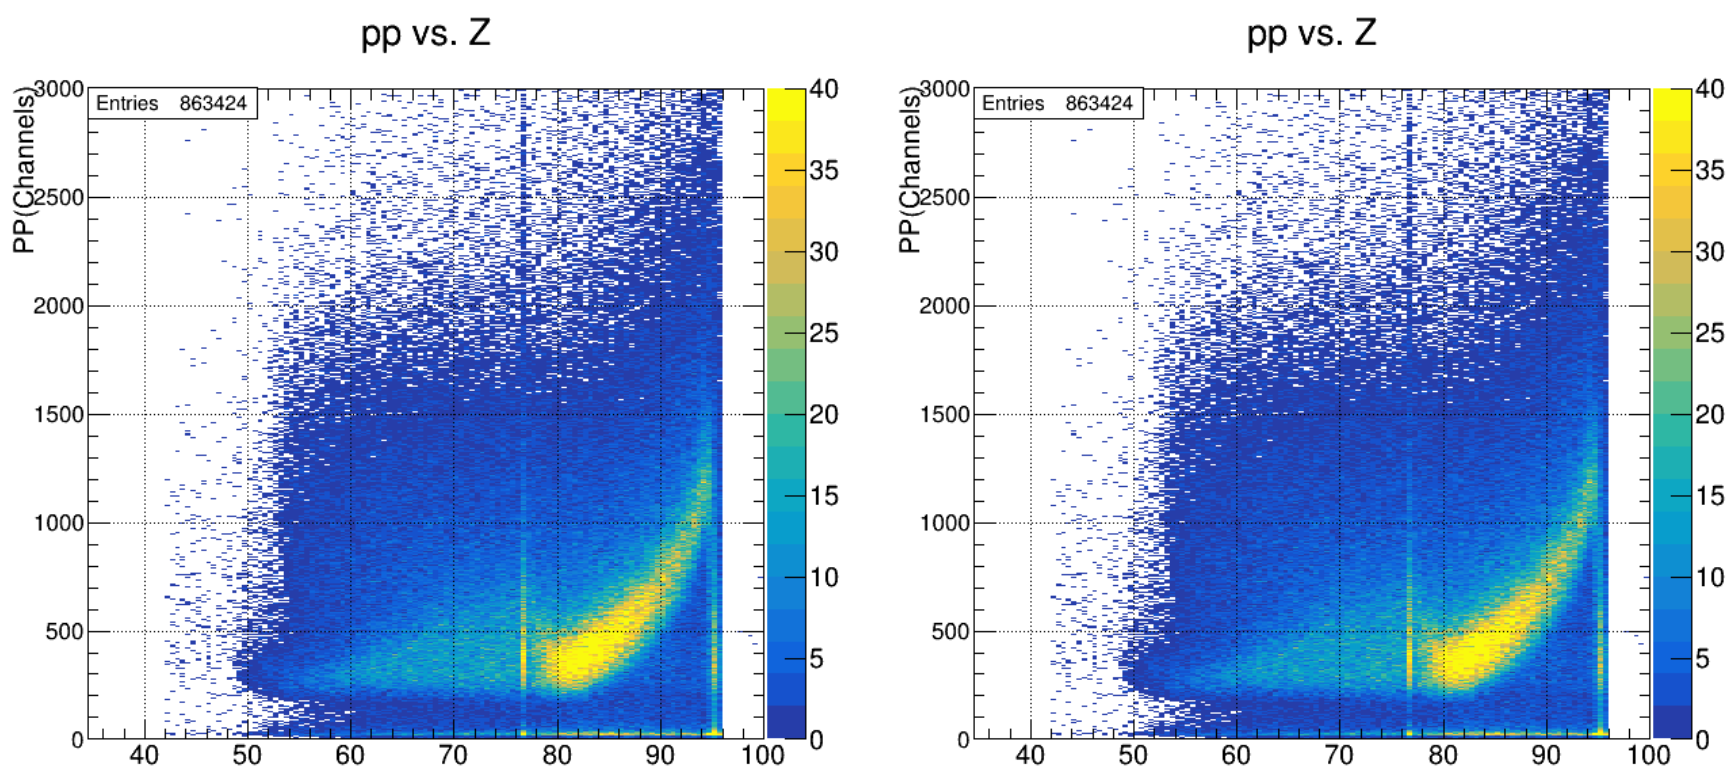
\includegraphics[width=1.0\columnwidth]{performance/figs/pi_pp_vs_zint}
		\caption{FADC spectra from the Spring 2017 run. Left: pulse integral versus the z-intersection of charged tracks matched to the ST. Right: pulse amplitude versus the z-intersection of charged tracks matched to the ST. The straight section corresponds to $40\ \mathrm{cm} < z < 80\ \mathrm{cm}$, the bend section $80\ \mathrm{cm} < z < 84\ \mathrm{cm}$, and the nose section $84\ \mathrm{cm} < z < 98\ \mathrm{cm}$.}
		\label{fig:pippvszint}
	\end{figure}
This feature of the ST geometry is quite advantageous since the majority of the charged tracks produced under the nominal \gx{} beam conditions intersect the ST in the nose region and therefore have the largest light amount of light collected by the SiPM's as the upstream end.

Once the proper attenuation corrections were applied to the data, the PID capabilities of the ST were greatly enhanced.  Figure ~\ref{fig:dEdx_vs_p_corr} illustrates the PID capability of charged tracks intersecting the ST.  As compared to Fig.~\ref{fig:dEdx_vs_p_uncorr}, the reliable separation of protons and other hadrons occurs for charged tracks with $p < 1.1\ GeV/c$ which is a factor two improvement from the uncalibrated data.
	\begin{figure}[!htb]
		\centering
		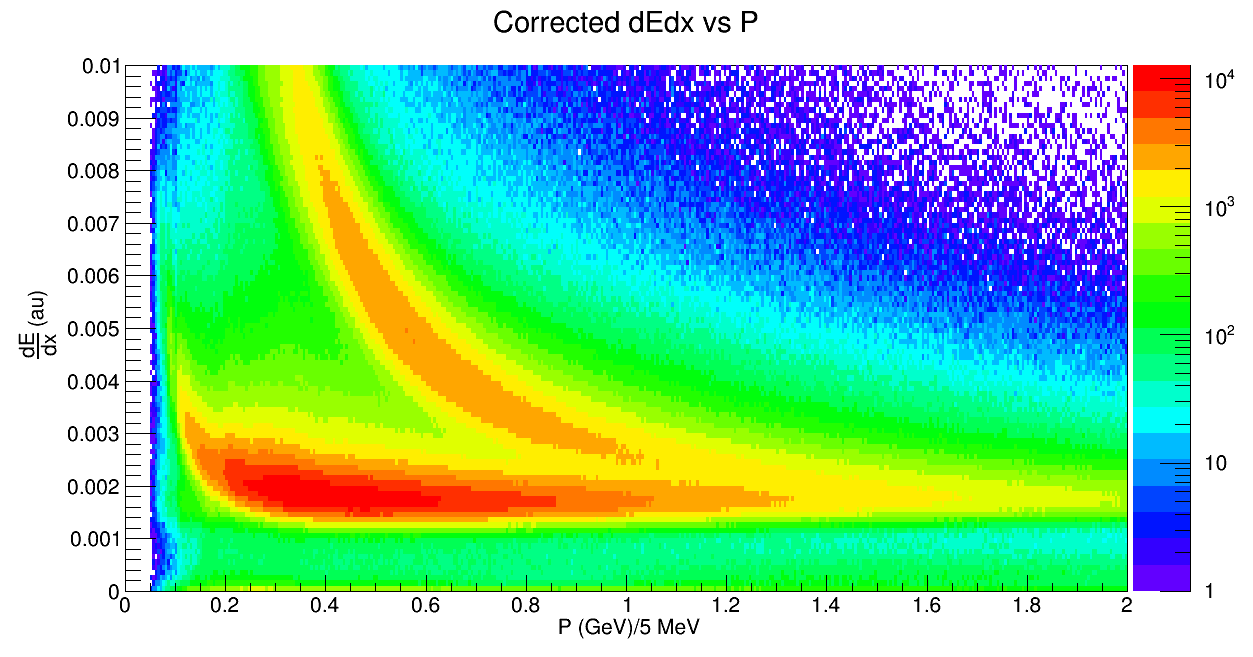
\includegraphics[width=1.0\columnwidth]{performance/figs/dEdx_vs_p_corr}
		\caption{Typical corrected $dE/dx\ vs.\ p$ distribution in the Start Counter.  Shown is the corrected $dE/dx\ vs.\ p$ distribution for tracks matched to the Start Counter in the Spring 2017 run. The ``banana band'' corresponds to protons while the horizontal band corresponds to charged electrons, pions, and kaons.  It is clear that pion/proton separation is achievable for tracks with $p < 1.1\ GeV/c$.}
		\label{fig:dEdx_vs_p_corr}
	\end{figure}  

After the previously discussed time-walk and propagation time corrections were complete, it was then possible to utilize the ST to measure the time of charged track vertices for tracks that are matched to the ST.  The vertex time is defined to be the time in which a polarized Bremsstrahlung photon interacted with the $\mathrm{LH_{2}}$ target and produced a charged track that intersected the ST.  An identical charged track selection process as outlined in Sec.~\ref{sec:calib_ptc} was utilized so that the time resolution of tracks matched to the ST could be measured.

The equation to calculate the ST measure of the vertex time is given by Eq.~\ref{eq:st_prop_time}.  In an identical manner outlined in Sec.~\ref{sec:calib_ptc}, $T^{RF}_{vertex}$ must be ``stepped'' to the time the charged track vertex was produced so as to obtain a proper measure of the RF time.  The resulting distribution in the time difference of these two times provides a measure of the ST time resolution and is seen in Fig. \ref{fig:beam_tof_corr_chan_15}.
	\begin{figure}[!htb]
		\centering
		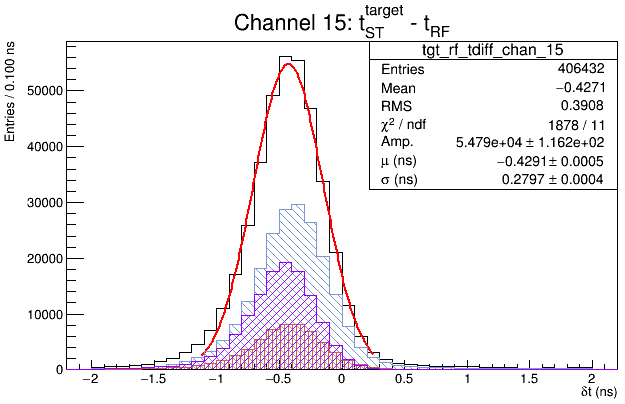
\includegraphics[width=0.7\linewidth]{performance/figs/beam_tof_corr_chan_15}
		\caption[Typical Start Counter/RF time resolution distribution]{Typical Start Counter/RF time resolution distribution.  Shown is the time resolution distribution for sector 15 during the Spring 2015 run 2931. The x-axis is the time difference between $T^{ST}_{vertex}$ and $T^{BB}_{vertex}$. The blue histogram is the resolution in the straight section. The red and purple histograms correspond to the resolution in the bend and nose sections respectively. The black histogram is a sum of the three sections and corresponds to the resolution along the entire length of the paddle.}
		\label{fig:beam_tof_corr_chan_15}
	\end{figure}

The aforementioned fits were then carried out for each of the ST sectors with $\sigma$, and its associated error being calculated.  Then a weighted average of the 30 $\sigma$'s were calculated so that the ST could have its time resolution characterized in its entirety.  The same procedure was also conducted for the three individual sections.  Figure \ref{fig:timeresallinset} illustrates the uniformity in time resolution among all sectors of the ST.
	\begin{figure}[!htb]
		\centering
		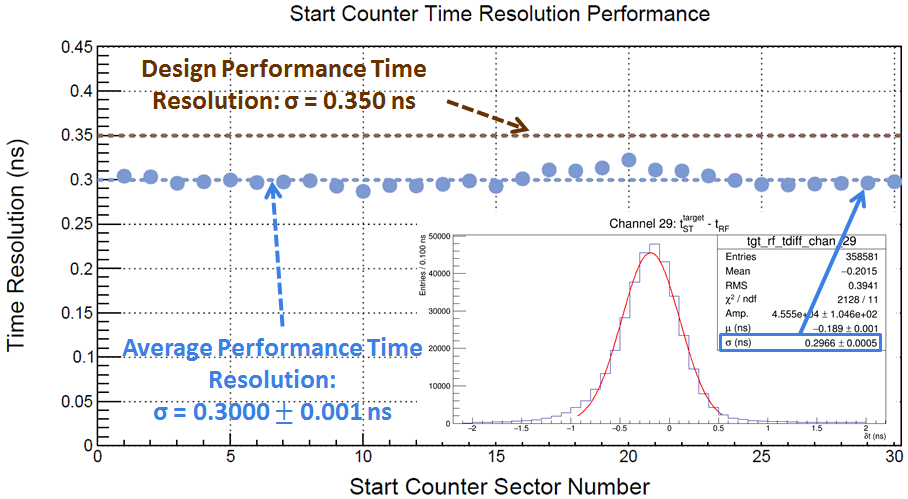
\includegraphics[width=1.0\columnwidth]{performance/figs/time_res_all_inset}
		\caption{ST time resolutions as a function of sector number. The inset illustrates a 2~$\sigma$ Gaussian fit the the ST time minus the RF time. The resulting $\sigma$ of the fit provides a measure of the time resolution.}
		\label{fig:timeresallinset}
	\end{figure}

Figure \ref{fig:timeresallinset} indicates that the average time resolution of 300~ps is well below the design resolution of 350~ps.  Table \ref{tab:time_res_section} details the weighted average time resolution of all the ST sectors in the different geometrical regions.
\begin{table}[ch]
	\centering
	\begin{tabular}{|c|c|c|c|c|}
		\hline  \textbf{Section} & $\mathbf{\sigma_{all}}$ & $\mathbf{\sigma_{straight}}$ & $\mathbf{\sigma_{bend}}$ & $\mathbf{\sigma_{nose}}$ \\ 
		\hline $\mathbf{\sigma_{avg}}$ & 290 ps & 299 ps & 292 ps & 264 ps \\ 
		\hline 
	\end{tabular}
	\caption[Average time resolutions by section]{Average time resolutions by section. Shown is the average of all 30 ST sectors by independent geometrical regions.}
	\label{tab:time_res_section}
\end{table}
It is clear from Table \ref{tab:time_res_section} that what is observed is that measurements made with beam data exhibit the same phenomenon of substantial improvement in light collection, and thus time resolution, as light is produced further downstream in the nose region.

When these time resolution measurements were conducted with data collected in Spring 2017, approximately 3 years had elapsed since the paddles were first tested on the bench at FIU.  Prior experience with degrading scintillators indicates that degradation in time resolution will be visible in a matter of weeks.  However, after 3 years no degradation has been observed and the ST is still performing well below design resolution.

%%WB edits
\section{Conclusion} \label{sec:conclusion}

The \gx{} Start Counter was designed and constructed at Florida International University for use in Hall-D at TJNAF to provide separation of the 500 MHz photon beam bunch structure delivered by the CEBAF to within 94\% accuracy.  It is the first ``start counter'' detector to have utilized magnetic field insensitive SiPMs as the readout system.  Despite the many design and manufacturing complications, the ST has proven to have performed well beyond the design timing resolution of 350~ps with an average measured resolution of 280~ps.  Furthermore, the capabilities of the ST make it a viable candidate to assist in PID calculations.

The unique geometry of the ST nose section has illustrated the advantage of tapering trapezoidal geometry in thin scintillators.  Through simulation, tests on the bench, and analysis of data obtained with beam it has been definitively demonstrated that this geometry results in a phenomenon in which the amount of light detected increases as the scintillation source moves further downstream from the readout detector.

Since it's installation in Hall-D during the Fall 2014 commissioning run, the ST has shown no measurable signs of deterioration in performance.  This suggests that the ST scintillators are void of crazing and will most likely be able to meet and exceed the design performance well beyond the scheduled run periods associated with the \gx{} experiment.

It is planned to incorporate the ST into the level 1 trigger of the \gx{} experiment for high luminosity $(> 0.5\ \mu A)$ running.  Preliminary studies suggest that the high efficiency $(> 95\%)$ of the ST, in combination with the calorimeters, provides good suppression of electromagnetic background in regards to the level 1 trigger.  Furthermore, the ST's high degree of segmentation has shown to suppress various background contributions associated with complex topologies while simultaneously providing precision timing information for reconstructed charged particles in \gx{}.%WB some edits
\section{Acknowledgments}

The authors would like to graciously thank the plethora of Jefferson Lab staff members in both the Engineering division and Hall-D.  Their numerous and invaluable contributions allowed for the Start Counter project to come to fruition.  The authors would also like to extend their gratitude to the entire \gx{} Collaboration who provided fruitful ideas and advice throughout the many stages of the project.  Work at Florida International University was supported in part by the Department of Energy under contracts DE–FG02–99ER41065 and DE-­SC0013620. Furthermore, this material is based upon work supported by the U.S. Department of Energy, Office of Science, Office of Nuclear Physics under Contract No.DE-AC05-06OR23177. 
\endgroup

\newpage
\section*{References}
\bibliography{bibliography/bibliography}

\end{document}